\documentclass[]{article}
\usepackage{lmodern}
\usepackage{amssymb,amsmath}
\usepackage{ifxetex,ifluatex}
\usepackage{fixltx2e} % provides \textsubscript
\ifnum 0\ifxetex 1\fi\ifluatex 1\fi=0 % if pdftex
  \usepackage[T1]{fontenc}
  \usepackage[utf8]{inputenc}
\else % if luatex or xelatex
  \ifxetex
    \usepackage{mathspec}
  \else
    \usepackage{fontspec}
  \fi
  \defaultfontfeatures{Ligatures=TeX,Scale=MatchLowercase}
\fi
% use upquote if available, for straight quotes in verbatim environments
\IfFileExists{upquote.sty}{\usepackage{upquote}}{}
% use microtype if available
\IfFileExists{microtype.sty}{%
\usepackage{microtype}
\UseMicrotypeSet[protrusion]{basicmath} % disable protrusion for tt fonts
}{}
\usepackage[margin=1in]{geometry}
\usepackage{hyperref}
\hypersetup{unicode=true,
            pdfborder={0 0 0},
            breaklinks=true}
\urlstyle{same}  % don't use monospace font for urls
\usepackage{longtable,booktabs}
\usepackage{graphicx,grffile}
\makeatletter
\def\maxwidth{\ifdim\Gin@nat@width>\linewidth\linewidth\else\Gin@nat@width\fi}
\def\maxheight{\ifdim\Gin@nat@height>\textheight\textheight\else\Gin@nat@height\fi}
\makeatother
% Scale images if necessary, so that they will not overflow the page
% margins by default, and it is still possible to overwrite the defaults
% using explicit options in \includegraphics[width, height, ...]{}
\setkeys{Gin}{width=\maxwidth,height=\maxheight,keepaspectratio}
\IfFileExists{parskip.sty}{%
\usepackage{parskip}
}{% else
\setlength{\parindent}{0pt}
\setlength{\parskip}{6pt plus 2pt minus 1pt}
}
\setlength{\emergencystretch}{3em}  % prevent overfull lines
\providecommand{\tightlist}{%
  \setlength{\itemsep}{0pt}\setlength{\parskip}{0pt}}
\setcounter{secnumdepth}{0}
% Redefines (sub)paragraphs to behave more like sections
\ifx\paragraph\undefined\else
\let\oldparagraph\paragraph
\renewcommand{\paragraph}[1]{\oldparagraph{#1}\mbox{}}
\fi
\ifx\subparagraph\undefined\else
\let\oldsubparagraph\subparagraph
\renewcommand{\subparagraph}[1]{\oldsubparagraph{#1}\mbox{}}
\fi

%%% Use protect on footnotes to avoid problems with footnotes in titles
\let\rmarkdownfootnote\footnote%
\def\footnote{\protect\rmarkdownfootnote}

%%% Change title format to be more compact
\usepackage{titling}

% Create subtitle command for use in maketitle
\providecommand{\subtitle}[1]{
  \posttitle{
    \begin{center}\large#1\end{center}
    }
}

\setlength{\droptitle}{-2em}

  \title{}
    \pretitle{\vspace{\droptitle}}
  \posttitle{}
    \author{}
    \preauthor{}\postauthor{}
    \date{}
    \predate{}\postdate{}
  
\usepackage{pdfcomment}
\usepackage{xcolor}
\usepackage{graphicx}
\usepackage{marginnote}

\begin{document}

\#Lecture3: (Chapter 3) Demand Curves

\#\#Discussion question

\begin{quote}
the price of beans went up, so people started buying more beans
\end{quote}

\bigskip

\textcolor{blue}{Could this ever be true? Is there a logical economic justification for this?}

\textcolor{gray}{Discuss with your neighbour... we will vote}

\hypertarget{lecture-3-chapter-3-demand-curves-key-goals}{%
\subsection{Lecture 3 (Chapter 3): Demand Curves -- key
goals}\label{lecture-3-chapter-3-demand-curves-key-goals}}

\begin{enumerate}
\def\labelenumi{\arabic{enumi}.}
\item
  To derive \emph{individual's} demand curve from her utility function
\item
  What properties do demand curves have?
\end{enumerate}

. . .

\begin{enumerate}
\def\labelenumi{\arabic{enumi}.}
\setcounter{enumi}{2}
\tightlist
\item
  Understand (\& derive) related concepts/outcomes:

  \begin{itemize}
  \tightlist
  \item
    Substitution and income effects (of a price change)
  \item
    Goods that are `substitutes' or `complements'
  \item
    \ldots{} Normal and inferior goods; Giffen goods
  \item
    Consumer surplus (from a transaction)
  \item
    The lump-sum principle (and the distortion of taxation)
  \end{itemize}
\end{enumerate}

. . .

\begin{enumerate}
\def\labelenumi{\arabic{enumi}.}
\setcounter{enumi}{3}
\tightlist
\item
  What is a \emph{market} demand curve, and how do we derive it?
\end{enumerate}

\begin{center}\rule{0.5\linewidth}{\linethickness}\end{center}

\begin{itemize}
\item
  \begin{enumerate}
  \def\labelenumi{\arabic{enumi}.}
  \setcounter{enumi}{3}
  \tightlist
  \item
    Understand the concepts and how to compute:
  \end{enumerate}

  \begin{itemize}
  \tightlist
  \item
    Price elasticity (of market demand for a product), and what it means
    to firms' pricing strategy
  \item
    Income elasticity (\ldots)
  \item
    Cross-price elasticity (between two products)
  \end{itemize}
\item
  \begin{enumerate}
  \def\labelenumi{\arabic{enumi}.}
  \setcounter{enumi}{4}
  \tightlist
  \item
    Learn to discuss real world applications of the above
  \end{enumerate}
\end{itemize}

\#\#Demand functions

\begin{itemize}
\tightlist
\item
  Previous: consumption choices determined by utility
  functions/indifference curves and budget constraints
\end{itemize}

. . .

\[Quantity \: of \: X \: demanded = d_x(P_X, P_Y, I; preferences)\]

\pdfnote{LC: Write this on the board}

\begin{center}\rule{0.5\linewidth}{\linethickness}\end{center}

\#\#\#Homogeneity

\begin{description}
\tightlist
\item[Homogeneous (of degree zero) (demand) function]
A function whose outcome value does not change when all arguments are
changed proportionally
\end{description}

. . .

\bigskip

\(d_X(P_X,P_Y,I)\) is homogenous in its arguments

\bigskip

\begin{itemize}
\tightlist
\item
  Multiply all prices and income by same amount \(\rightarrow\) budget
  constraint unchanged \(\rightarrow\) consumption choices the same
\end{itemize}

. . .

\begin{itemize}
\tightlist
\item
  E.g., \(P_X X + P_Y Y = I\) is the same as \(2P_X X + 2P_Y Y = 2I\)
\end{itemize}

\pdfnote{Intuition: Graphically, the budget line and indifference curves are unchanged, so the point of tangency is the same. \textCR
 Consider, if your income, as well as prices, were stated in pennies rather than pounds (e.g., 5 million pennies rather than \pounds50,000), why would your choices change?}

\pdfnote{This relates to the puzzle of 'why should monetary policy and inflation have any real effect?'}

\begin{center}\rule{0.5\linewidth}{\linethickness}\end{center}

\#\#Response to income changes

\[d_x(P_X, P_Y, I; preferences)\]

\bigskip

\begin{itemize}
\tightlist
\item
  What happens to the quantity purchased of some good as your income
  increases?
\end{itemize}

\pdfnote{LC: Ask this as class question}

. . .

\begin{itemize}
\tightlist
\item
  Depends on whether the good is \emph{normal} or \emph{inferior}
\end{itemize}

\bigskip

\pdfnote{Whether it is normal or inferior depends on your preferences and the change in the slope of the indifference curves with higher income/utility, as we see below}

\begin{description}
\tightlist
\item[Normal good]
A good that is bought in greater quantities as income increases.
\item[Inferior good]
A good that is bought in smaller quantities as income increases.
\end{description}

\begin{center}\rule{0.5\linewidth}{\linethickness}\end{center}

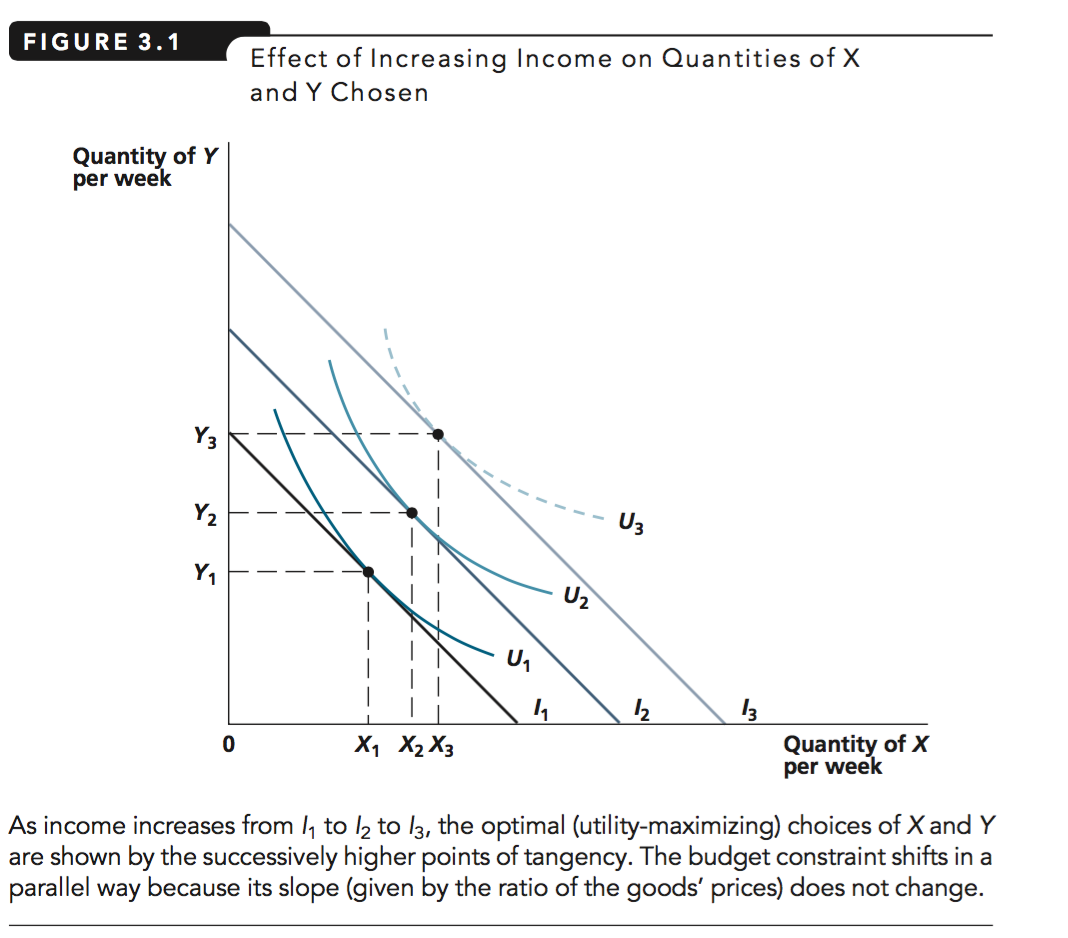
\includegraphics[height=4in]{picsfigs/normalgood.png}

\pdfnote{Two things going on here: \textCR
1. A wider set of consumption possibilities ... can afford more of X for any Y and v/v \textCR
2. At higher levels of consumption and utility the psychic tradeoffs (mrs) may change}

\begin{center}\rule{0.5\linewidth}{\linethickness}\end{center}

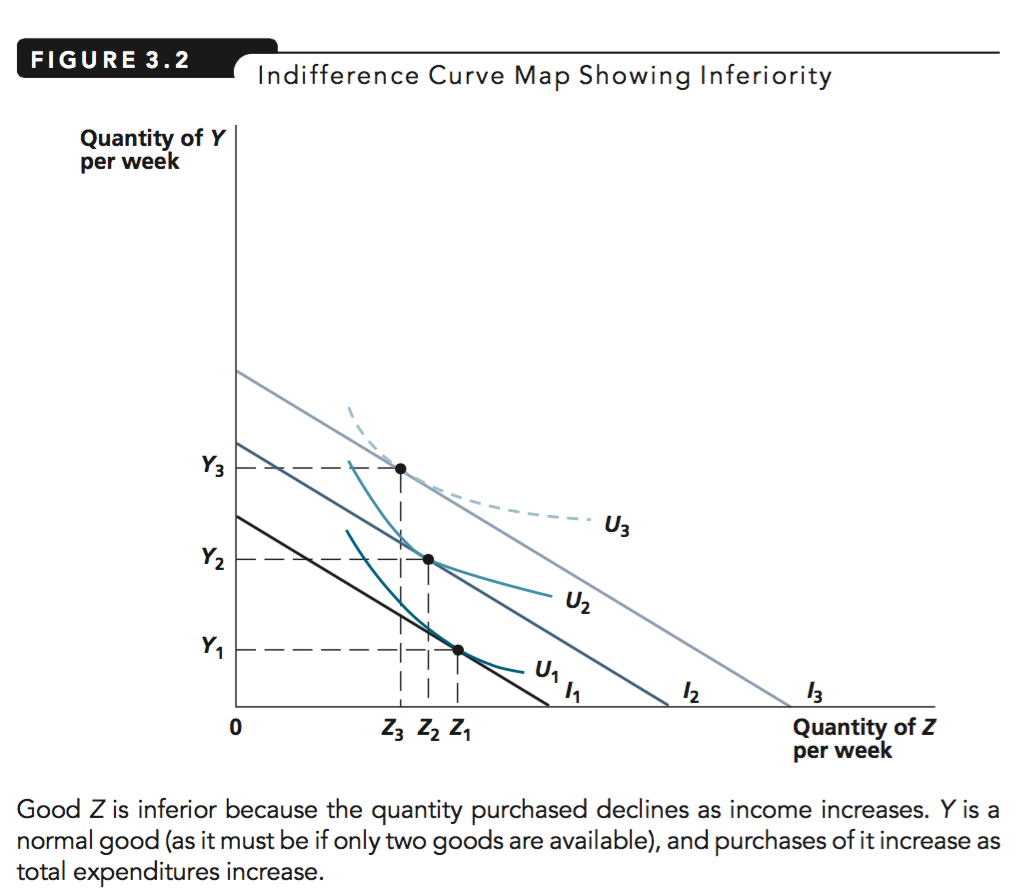
\includegraphics{picsfigs/inferiorgood.png}\\

\pdfnote{More income, less expenditure on Z? \textCR
It's bc the shape of indifference curves differs at higher incomes here; shallower. \textCR
When people have a lot to spend, they want to spend it on Y and not on Z. \textCR
If you won the lottery how much pot noodle would you buy?}

\pdfnote{Adv: To be precise, it's *not* about wealthy people being different than poor people \textCR
... We're considering the *same* person with higher income.
Thinking in 3d: 'as you walk up this hill, it's ridge gradually moves to the west'}

\pdfnote{Adv: Consider -- all goods cannot be inferior. Why not?}

\pdfnote{Move to PPT slides to illustrate this, \textCR
 beginning with 'Changes in Income: A Normal Good'}

\#\#Substitution and income effects from a fall (or rise) in price

\[d_x(P_X, P_Y, I; preferences)\]

\bigskip

What happens to the quantity purchased of some good when the price of
the good falls or rises?

\pdfnote{Changes both an intercept and a slope. \textCR
New utility-maximizing choice on *another* indifference curve is \textCR
 a point on that curve with a different MRS.}

. . .

\begin{description}
\tightlist
\item[Substitution effect (`Hicksian')]
The effect on consumption due to a change in price `holding utility
constant.'
\end{description}

\textcolor{gray}{Precisely: effect on the lowest-cost bundle yielding this utility}

. . .

\begin{description}
\tightlist
\item[Income effect (of a price change)]
The remaining effect on consumption; price change \(\rightarrow\) change
in purchasing power/achievable utility.
\end{description}

\pdfnote{This is conceptual: we never *actually* observe either of these effects alone; \textCR
 we always observe the net effect of both}

\pdfnote{Standard definition of the 'income effect' of a price change \textCR
combines both 'effects of an income change' we saw above \textCR
more consumption of each good is possible, but the MRS may differ at this higher utility}

\begin{center}\rule{0.5\linewidth}{\linethickness}\end{center}

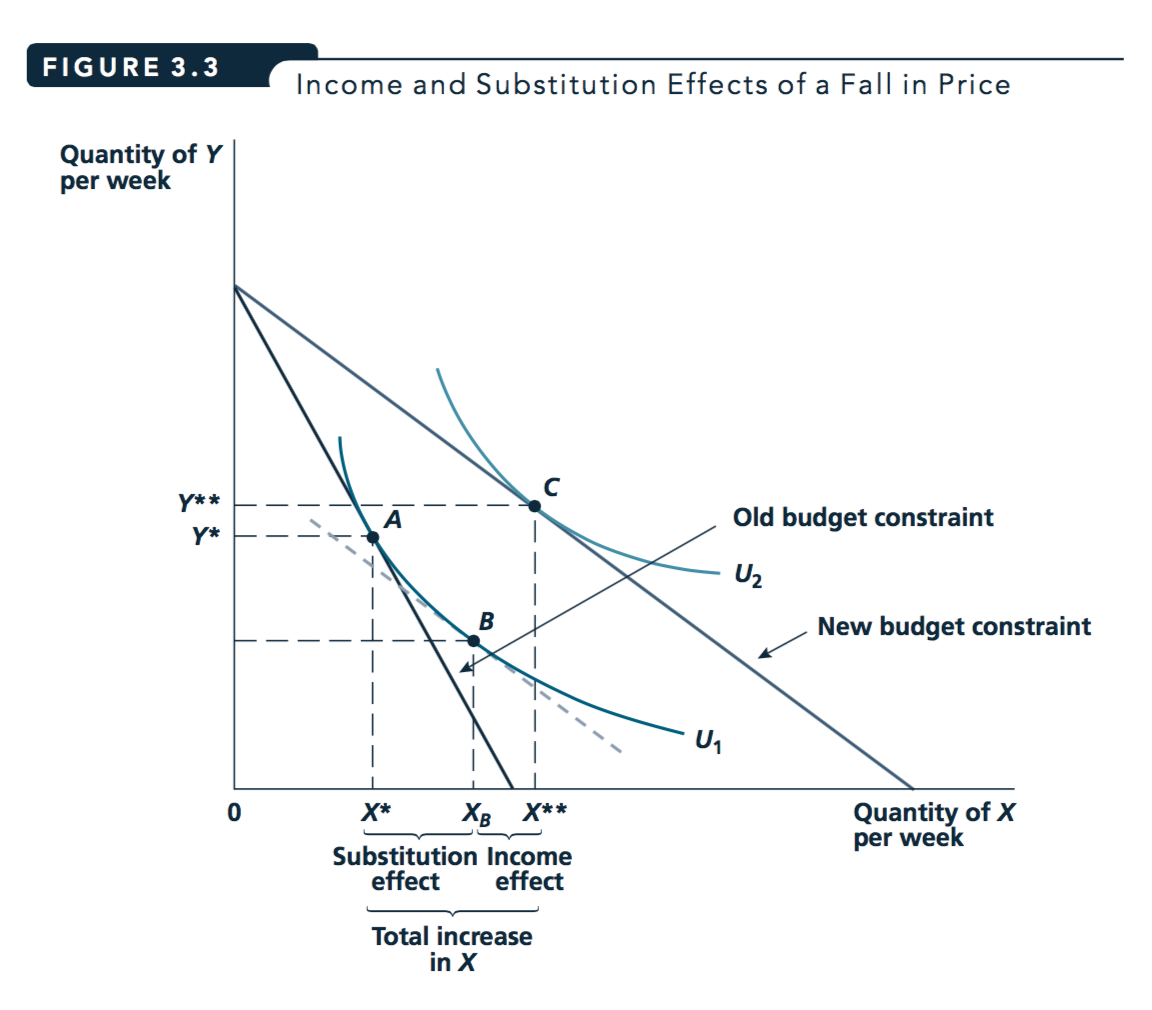
\includegraphics{picsfigs/incomeandsubstfx.png}\\

\pdfnote{Move to PPT slides to illustrate this, \textCR
 beginning with 'Change in A Good's Price'}

\pdfnote{Adv: This topic is more nuanced and complicated than we will cover in the main content of this module. \textCR
To fully cover this, we would have to consider the theoretical concept of a 'compensated' aka 'Hicksian' demand curve, \textCR
where income is adjusted to hold utility constant while price ratios change. \textCR
This also allows us to consider 'net versus gross' substitution, and 'equivalent vs compensating variation'. \textCR
More advanced economics modules will cover this extensively and rigorously.}

\begin{center}\rule{0.5\linewidth}{\linethickness}\end{center}

\begin{itemize}
\tightlist
\item
  Substitution effect:
  \textcolor{blue}{\underline{always} opposite direction as price change}
\end{itemize}

\pause

\begin{itemize}
\tightlist
\item
  Income effect

  \begin{itemize}
  \tightlist
  \item
    Normal good \(\rightarrow\)
    \textcolor{blue}{Opposite direction as price change}
  \item
    Inferior good: \textcolor{brown}{Same direction as price change}
    \pause
  \end{itemize}
\end{itemize}

\bigskip

Thus

\begin{itemize}
\tightlist
\item
  Normal good: Substitution \& income effects go in \emph{same
  direction}
\end{itemize}

\pause

\begin{itemize}
\tightlist
\item
  Inferior good: Substitution \& income effects go in opposite
  directions

  \begin{itemize}
  \tightlist
  \item
    \(\rightarrow\) \emph{Net} effect unknown
  \item
    Usually substitution effect dominates
    \textcolor{gray}{but see Giffen goods}
  \end{itemize}
\end{itemize}

\begin{center}\rule{0.5\linewidth}{\linethickness}\end{center}

\textbf{Read on your own, know:}

\begin{itemize}
\tightlist
\item
  Numerical example of response to price change
\item
  The relative importance of substitution effects for most goods
\item
  Substitution and income effects for inferior goods
\end{itemize}

\hypertarget{different-substitution-effects}{%
\subsection{Different substitution
effects}\label{different-substitution-effects}}

\begin{itemize}
\item
  Perfect complements: No substitution effect, only an income effect of
  a price change
\item
  Perfect substitutes: Large substitution effect -- price change may
  cause a complete switch
\item
  In between: depends on curvature of indifference curve
\end{itemize}

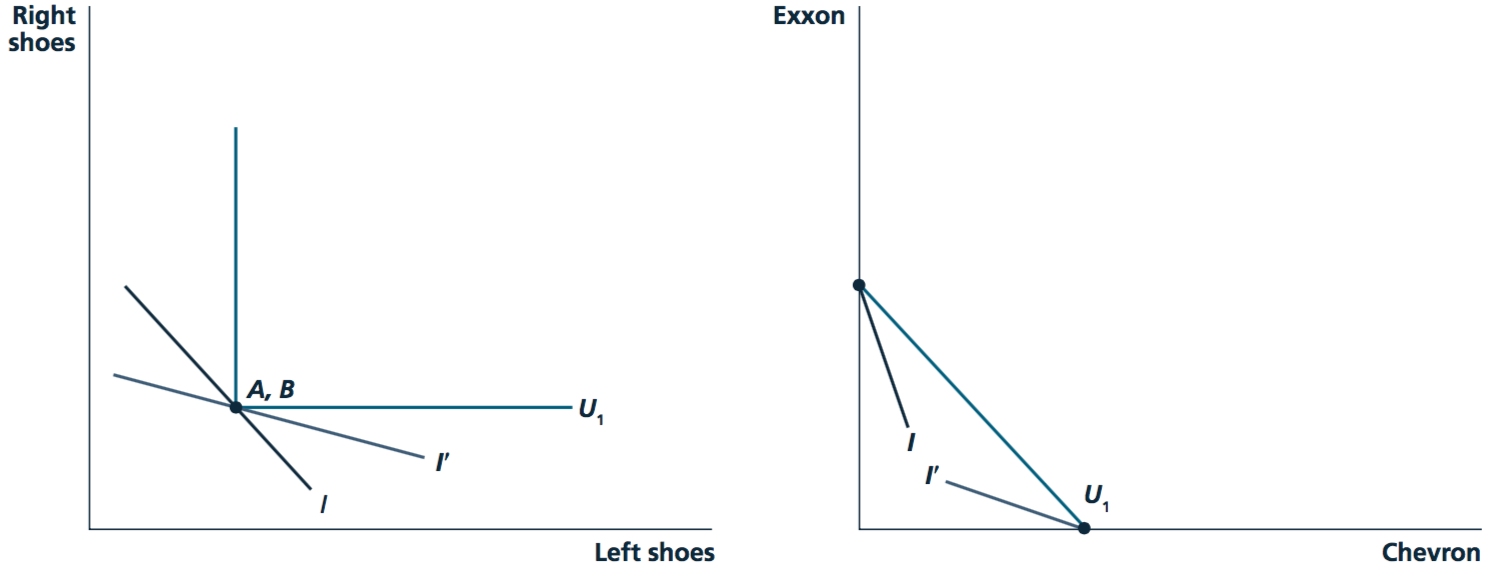
\includegraphics[height=3.5in]{picsfigs/substfxperfect_trim.png}

\begin{center}\rule{0.5\linewidth}{\linethickness}\end{center}

\hypertarget{the-legendary-giffen-good}{%
\subsection{The (legendary?) Giffen
good}\label{the-legendary-giffen-good}}


\includegraphics[height=2in]{picsfigs/griffin.jpg}

\begin{itemize}
\tightlist
\item
  If the price of a good increases, can quantity demanded actually
  \emph{increase}?!
\end{itemize}

. . .

\begin{itemize}
\tightlist
\item
  Yes, if the good is \emph{very} inferior and is a large portion of
  income
\end{itemize}

\pdfnote{
- But it has never been seen and documented in the wild \textCR
- See Powerpoint (if time permits) \textCR
- Practice question: try to draw indifference curves and budget constraints illustrating this effect for a Giffen good
}

\#\#Second lecture on demand \ldots{} WHAT???!!

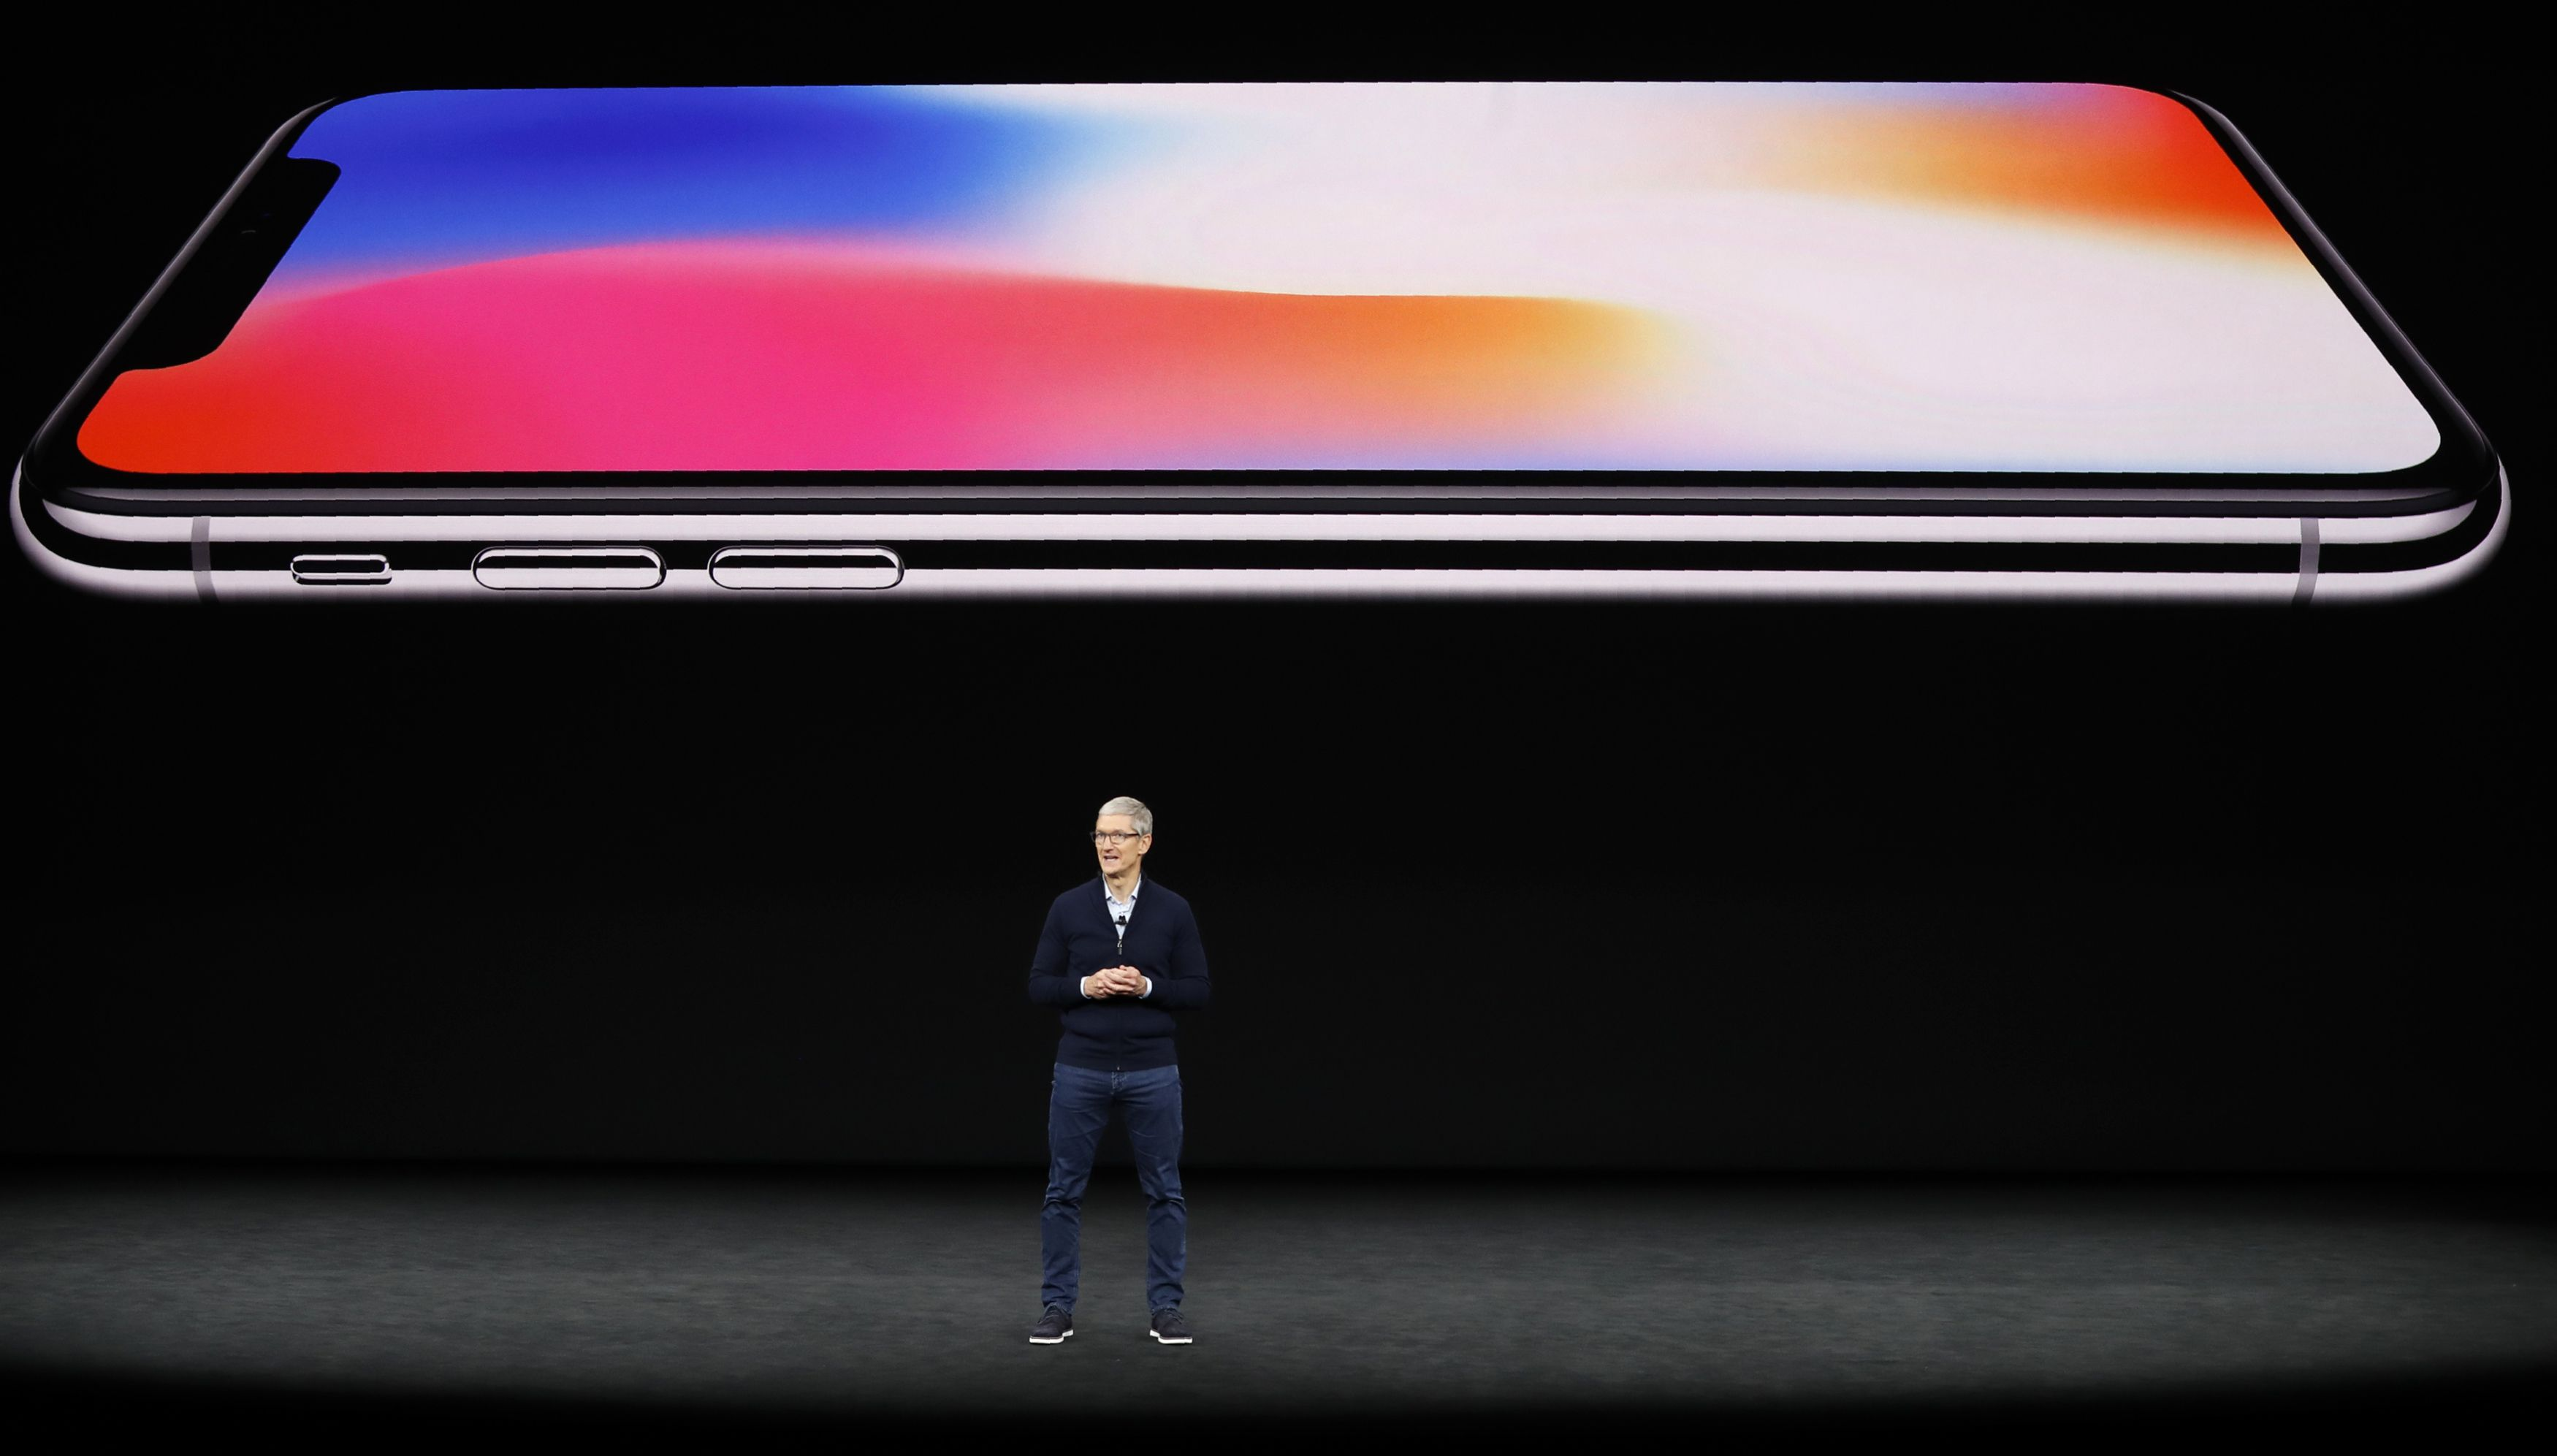
\includegraphics[height=3in]{picsfigs/iphonex.jpg}

\begin{center}\rule{0.5\linewidth}{\linethickness}\end{center}

Hands up please. If you could \emph{not} resell or gift it\ldots{}

\begin{itemize}
\tightlist
\item
  Would you accept a free IPhone X(s)?
\end{itemize}

. . .

Would you pay:

\begin{itemize}
\tightlist
\item
  250?
\end{itemize}

. . .

\begin{itemize}
\tightlist
\item
  500?
\end{itemize}

. . .

\begin{itemize}
\tightlist
\item
  750?
\end{itemize}

. . .

\begin{itemize}
\tightlist
\item
  1000?
\end{itemize}

. . .

\begin{itemize}
\tightlist
\item
  1250?
\end{itemize}

\begin{center}\rule{0.5\linewidth}{\linethickness}\end{center}

If your income was \pounds 100,000, would you pay

\begin{itemize}
\tightlist
\item
  500?
\end{itemize}

. . .

\begin{itemize}
\tightlist
\item
  750?
\end{itemize}

. . .

\begin{itemize}
\tightlist
\item
  1000?
\end{itemize}

. . .

\begin{itemize}
\tightlist
\item
  1250?
\end{itemize}

\begin{center}\rule{0.5\linewidth}{\linethickness}\end{center}

Back to your current income .. what if all other smartphones cost
\pounds 2000?

Would you pay for the Iphone X(s):

\begin{itemize}
\tightlist
\item
  500?
\end{itemize}

. . .

\begin{itemize}
\tightlist
\item
  750?
\end{itemize}

. . .

\begin{itemize}
\tightlist
\item
  1000?
\end{itemize}

. . .

\begin{itemize}
\tightlist
\item
  1250?
\end{itemize}

\#\#Second lecture on demand \ldots{} Recap

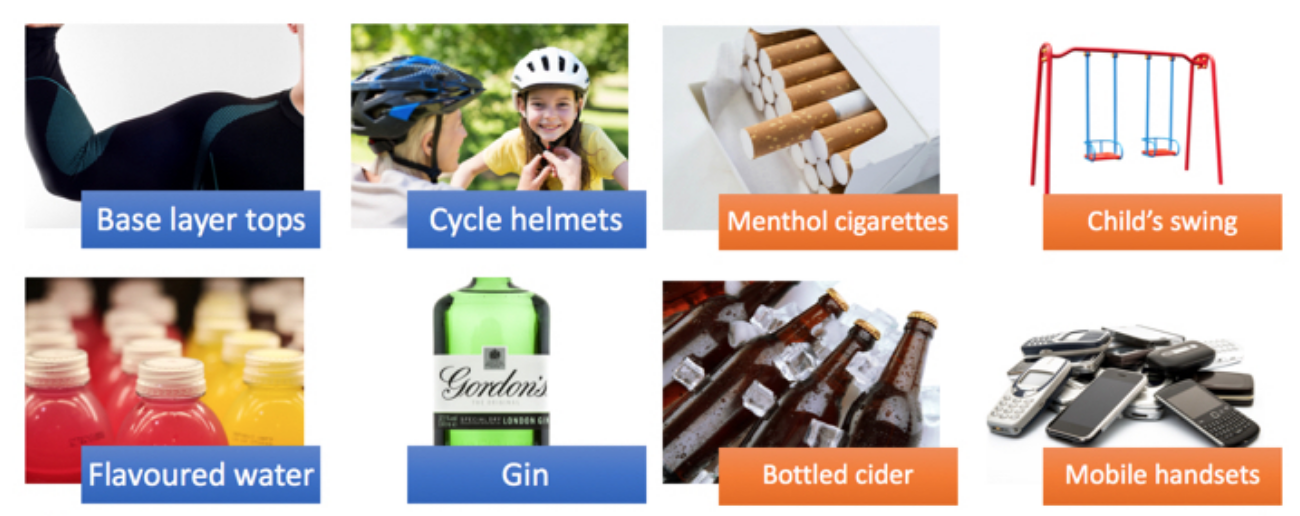
\includegraphics[height=3in]{picsfigs/ukcpi_inout.png}

\textcolor{blue}{What do these things have in common?}

\begin{center}\rule{0.5\linewidth}{\linethickness}\end{center}

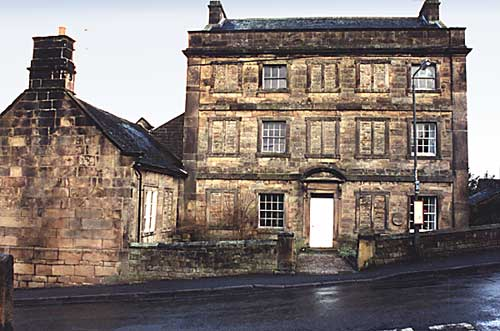
\includegraphics[height=3in]{picsfigs/ukwindows.jpg}

\textcolor{blue}{What explains this?}

\begin{center}\rule{0.5\linewidth}{\linethickness}\end{center}

\[Quantity \: of \: x \: demanded = d_x(p_x, p_y, I; preferences)\]

. . .

Previous lecture: What the constrained util-max implied for\ldots{}

\begin{itemize}
\item
  `Homogeneity of degree zero' of \(d_x(p_x, p_y, I)\)
\item
  How \(d_x\) responds to \(I\)
  \textcolor{gray}{(remember: inferior \& normal goods)}
\end{itemize}

. . .

\begin{itemize}
\item
  How \(d_x\) responds to \(P_x\)
  \textcolor{gray}{(rem: normal or Giffen)}

  \begin{itemize}
  \tightlist
  \item
    Substitution and income effects
  \end{itemize}
\end{itemize}

\#\#Goals: This lecture chunk (demand part 2)

\emph{Util-max s.t. constraints} \(\rightarrow\)

. . .

\textbf{Understand real-world issues:}

\begin{itemize}
\item
  `Fixed-basket' CPI may overstate inflation
\item
  Lump-sum principle, distortion of taxation
\end{itemize}

. . .

\textbf{Fundamental concepts, useful for business \& policy:}

\begin{itemize}
\item
  Goods that are `substitutes' or `complements'
\item
  Consumer surplus (from a transaction)
\end{itemize}

\begin{center}\rule{0.5\linewidth}{\linethickness}\end{center}

\ldots{}

\textbf{Derive}

\begin{itemize}
\item
  \emph{Individual's} demand curve from her utility function
\item
  \emph{Market} demand curve

  \begin{itemize}
  \tightlist
  \item
    \textcolor{gray}{What causes *shifts* in either?}
  \end{itemize}
\end{itemize}

\pause

\begin{itemize}
\tightlist
\item
  How to compare (the price and income elasticities) of apples and
  orange juice 
\end{itemize}

\begin{center}\rule{0.5\linewidth}{\linethickness}\end{center}

\#\#App 3.2: The CPI and it's biases

\pdfnote{Note UK also uses a similar CPI measure (since 2003, \textCR
 but RPI still used for some things). \textCR
 Bank of England targets 2\% increase in the CPI per year}

\begin{itemize}
\item
  A \emph{very} important number: Used for monetary policy and for
  targeting many salaries and benefits

  \begin{itemize}
  \tightlist
  \item
    But does it overstate the rate of inflation?
  \end{itemize}
\end{itemize}

\pause

Based on a `typical market basket'

\begin{itemize}
\tightlist
\item
  \textcolor{gray}{UK: of 700 different goods and services, excluding housing, updated yearly.}
\end{itemize}

\begin{center}\rule{0.5\linewidth}{\linethickness}\end{center}

A good example, 1982 vs 2012:

\[b_{82}=p^x_{82}x_{82}+p^y_{82}y_{82}\]
\[b_{12}=p^x_{12}x_{82}+p^y_{12}y_{82}\]
\[cpi_{12}=\frac{b_{12}}{b_{82}}\]

\begin{center}\rule{0.5\linewidth}{\linethickness}\end{center}

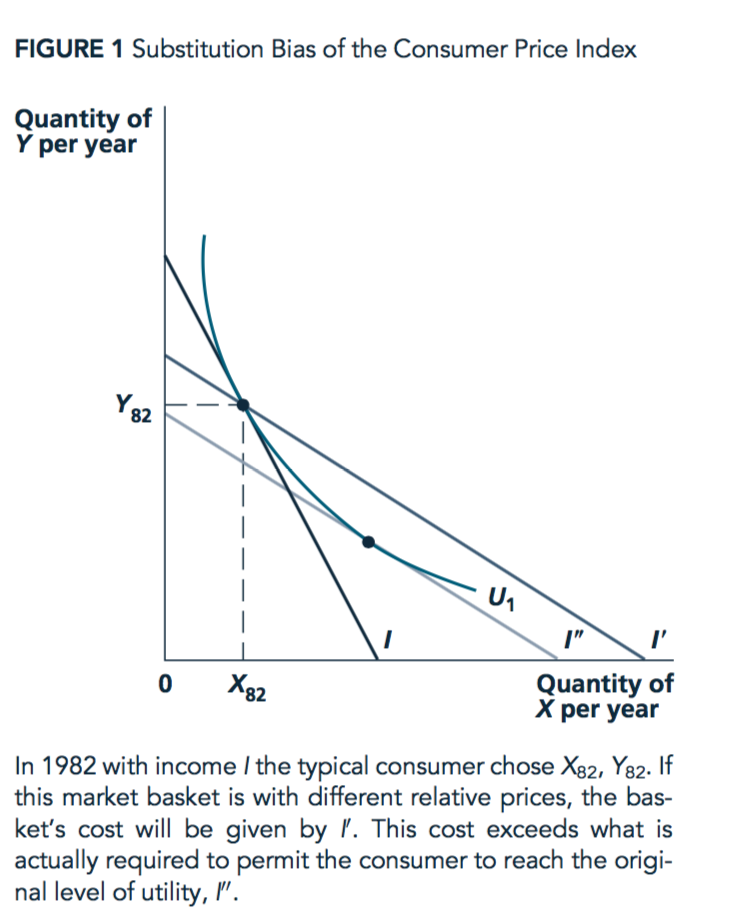
\includegraphics[height=3.7in]{picsfigs/cpi_bias.png}

\pdfnote{Unadjusted (fixed-basket, CPI 'claims' you need $I'$ to be as well off in 2012. \textCR
I.e., to buy *the exact same basket*, including vinyl records. \textCR
But by substituting, can get same utility w/ lower income $I''$ \textCR
(And $I'$  actually makes you *better* off).}

\pdfnote{Note basket *is* adjusted yearly, based on a household spending surveys. \textCR
But this also has problems: utility may be changing as people adjust their basket.\textCR
'Correct' adjustment depends on (unobservable) utility functions.}

\begin{center}\rule{0.5\linewidth}{\linethickness}\end{center}

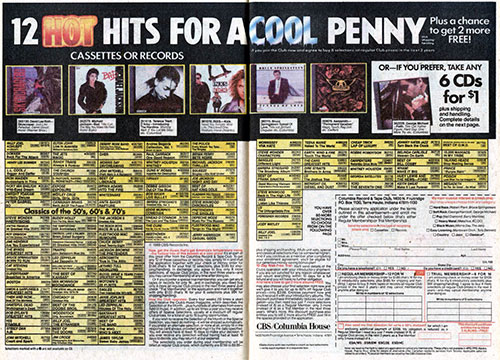
\includegraphics[height=3.5in]{picsfigs/12hitsforapenny.jpg}

\hypertarget{the-lump-sum-principle}{%
\subsection{The Lump-Sum Principle}\label{the-lump-sum-principle}}

\begin{figure}
\centering
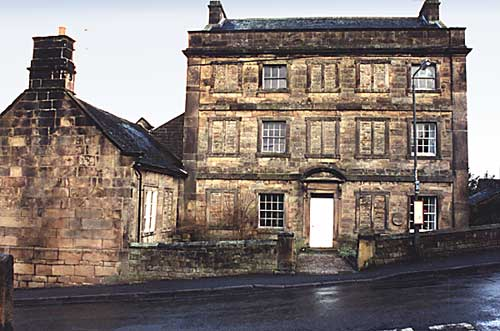
\includegraphics{picsfigs/ukwindows.jpg}
\caption{Have you seen this?}
\end{figure}

\pdfnote{1696: Act for granting to His Majesty several Rates or Duties upon Houses for \textCR
  making good the Deficiency of the clipped Money...  \textCR
Properties with 10-20 windows paid an extra 4 shillings (\pounds24.79 in 2016), \textCR
and those with 20+ windows paid extra 8 shillings (\pounds49.57 in 2016). <https://en.wikipedia.org/wiki/Window_tax>}

\pdfnote{Consider 'least efficient tax': UK government imposes a tax on all windows above 4 per house. \textCR
All residents bricks all windows above 4.  Government raises no revenue but people are certainly worse off.}

\begin{center}\rule{0.5\linewidth}{\linethickness}\end{center}

\begin{figure}
\centering
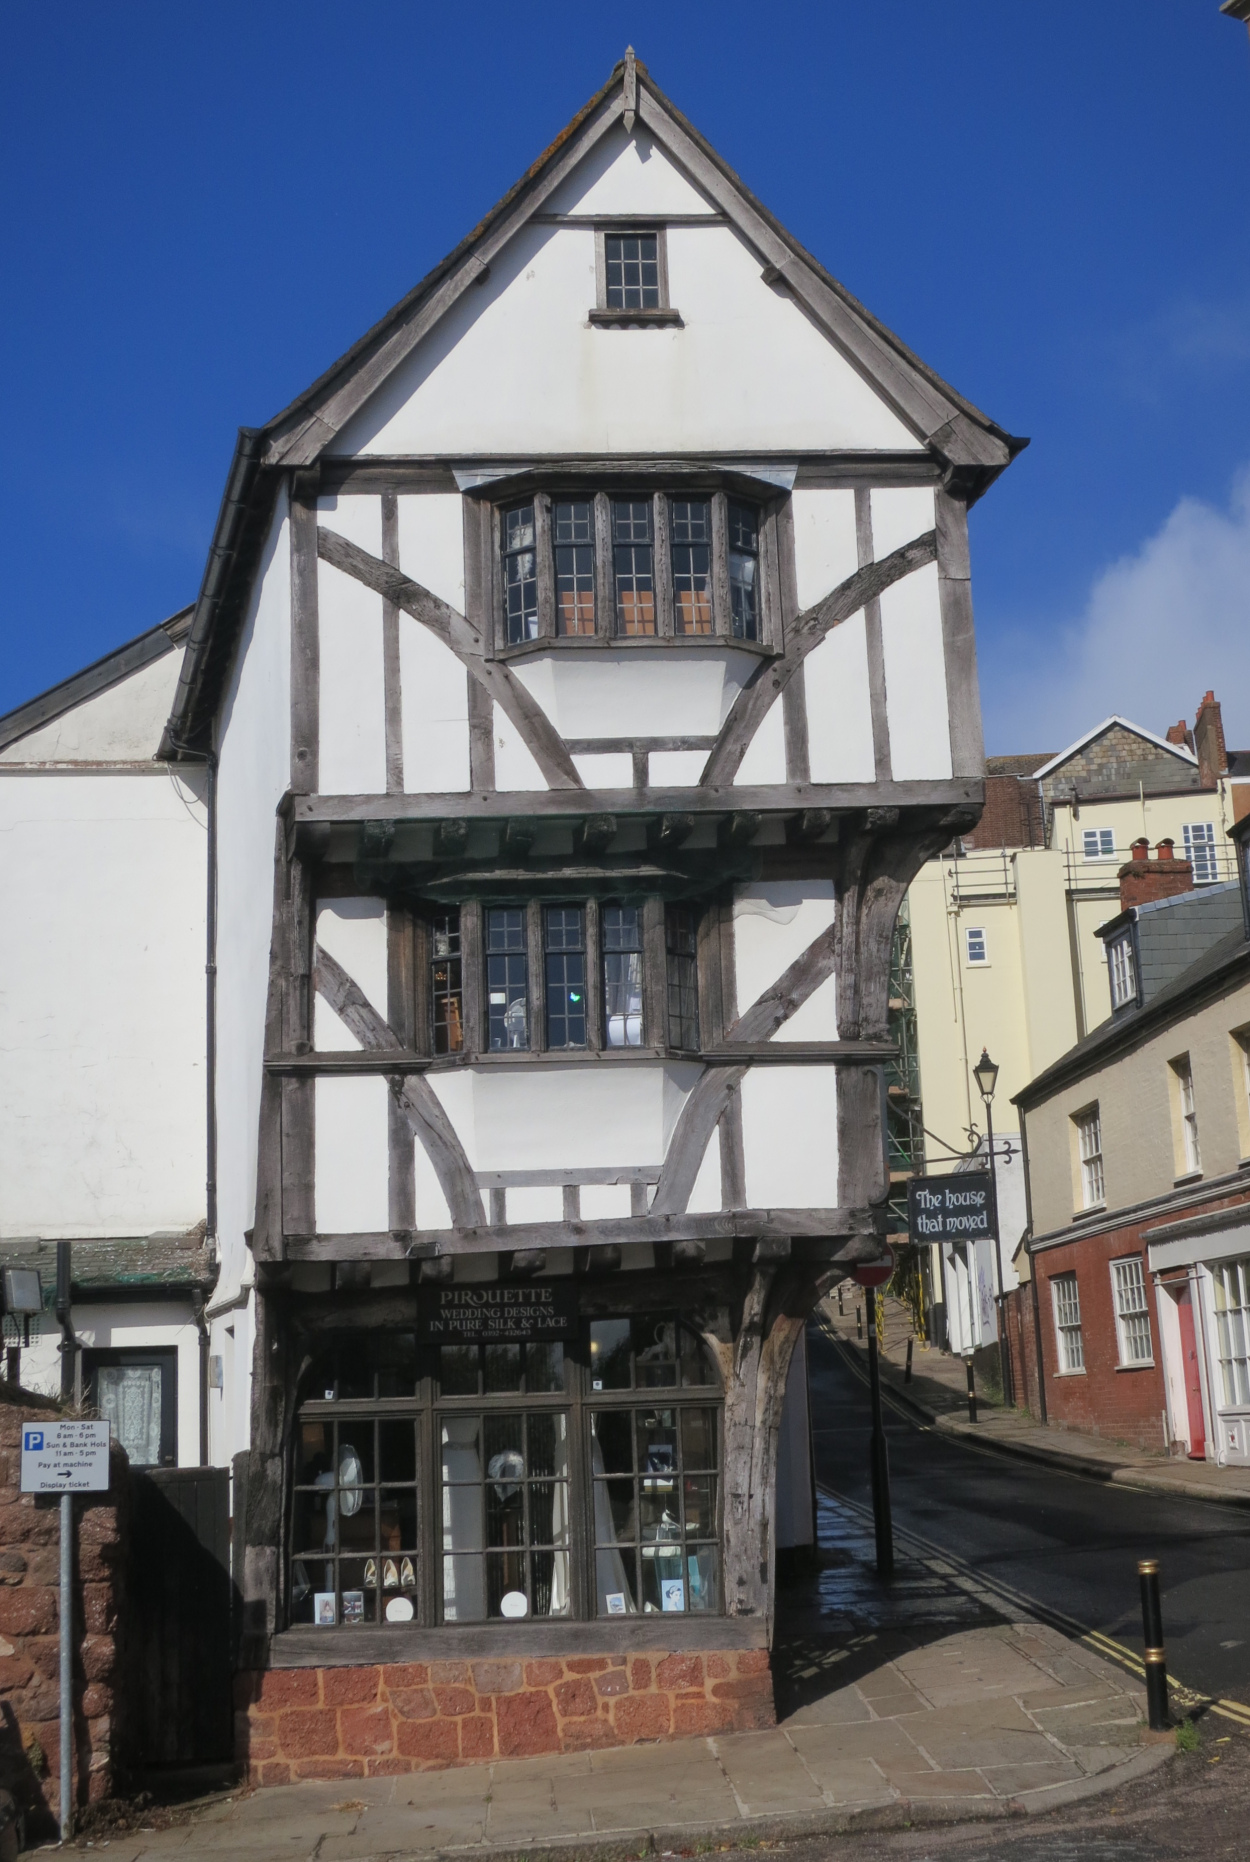
\includegraphics{picsfigs/tudoroverhang.jpg}
\caption{What's going on here?}
\end{figure}

\pdfnote{'Taxes based on ground-floor area' are mentioned throughout the web, but I couldn't find an authoritative reference to this. \textCR
 If anyone finds one, please let me know!}

\begin{center}\rule{0.5\linewidth}{\linethickness}\end{center}

\begin{itemize}
\tightlist
\item
  The social cost (deadweight loss) is greater the more taxes change
  `compensated' behaviour (via substitution)
\end{itemize}

\pdfnote{Why 'compensated' behavior?  \textCR
... bc taxes always leave people with less effective income, \textCR
causing consumption choices to reflect new, lower indifference curves. \textCR
For the DWL we care how taxes change their behavior *at this new lower-income*}

\pause

\begin{itemize}
\tightlist
\item
  The most efficient tax:

  \begin{itemize}
  \tightlist
  \item
    raises the most revenue for a given utility loss
  \item
    reduces utility the least for a given revenue
  \end{itemize}
\end{itemize}

\pause

\begin{itemize}
\tightlist
\item
  \ldots{} is a `lump-sum tax': same tax no matter what you do
  (including work/leisure!)

  \begin{itemize}
  \tightlist
  \item
    rationale for the poll tax
  \end{itemize}
\end{itemize}

\pdfnote{A common measure: 'amount person would be willing to pay to avoid tax' \textCR
for a given revenue raised}

\begin{center}\rule{0.5\linewidth}{\linethickness}\end{center}

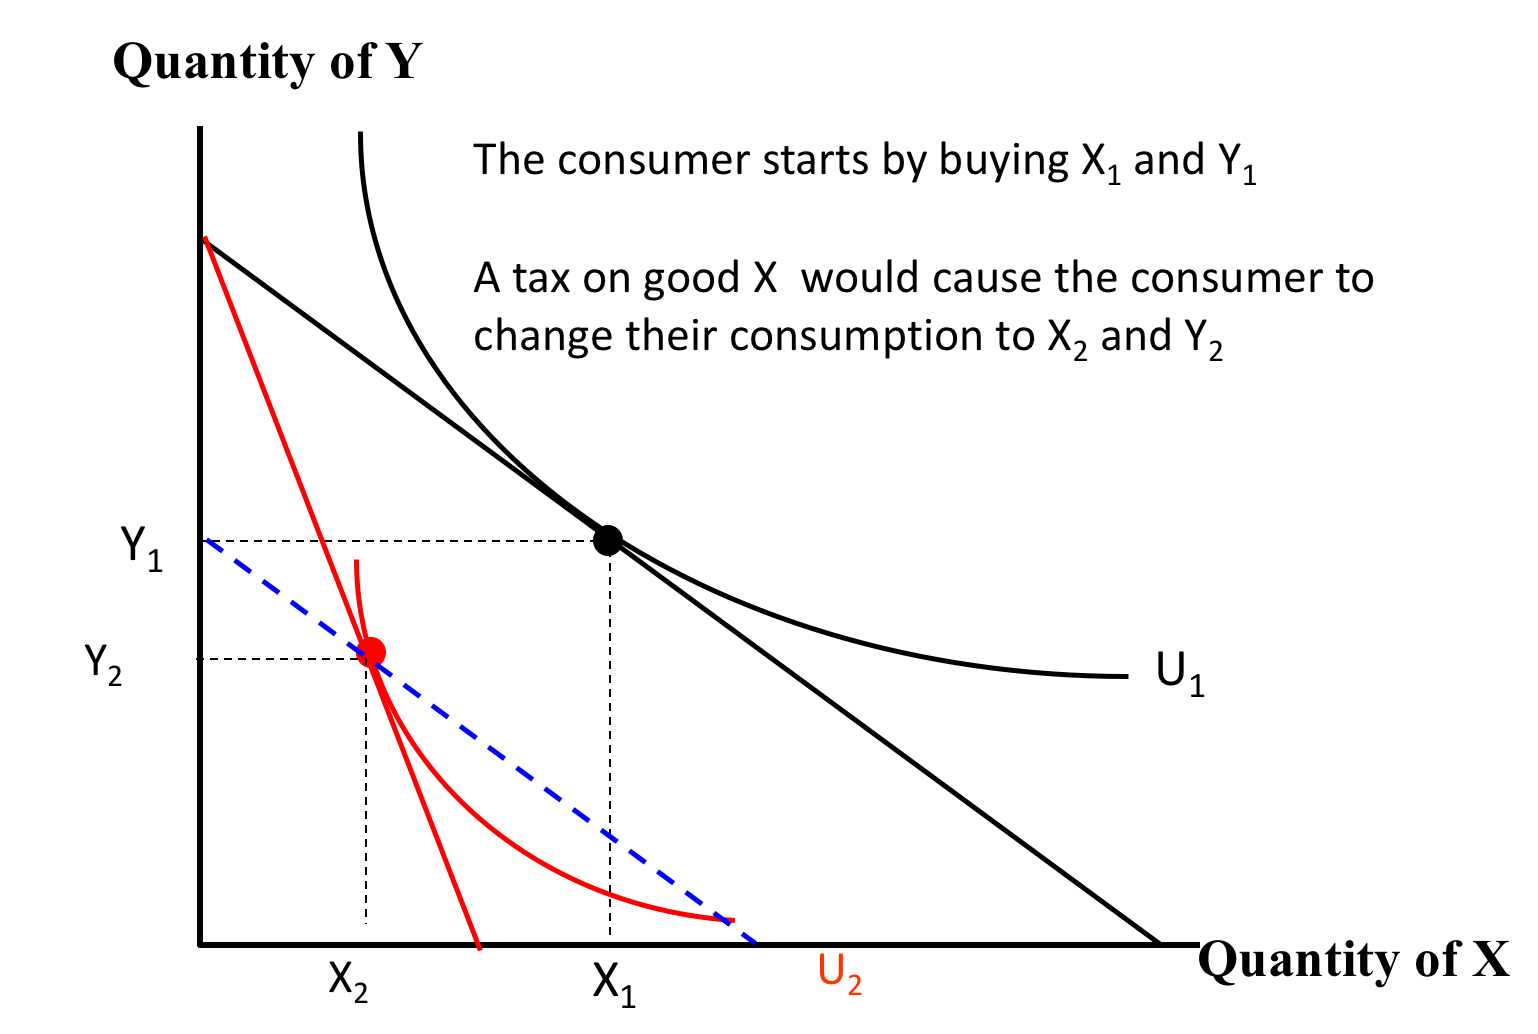
\includegraphics[height=3.3in]{picsfigs/taxwithblueline.png}

\begin{center}\rule{0.5\linewidth}{\linethickness}\end{center}

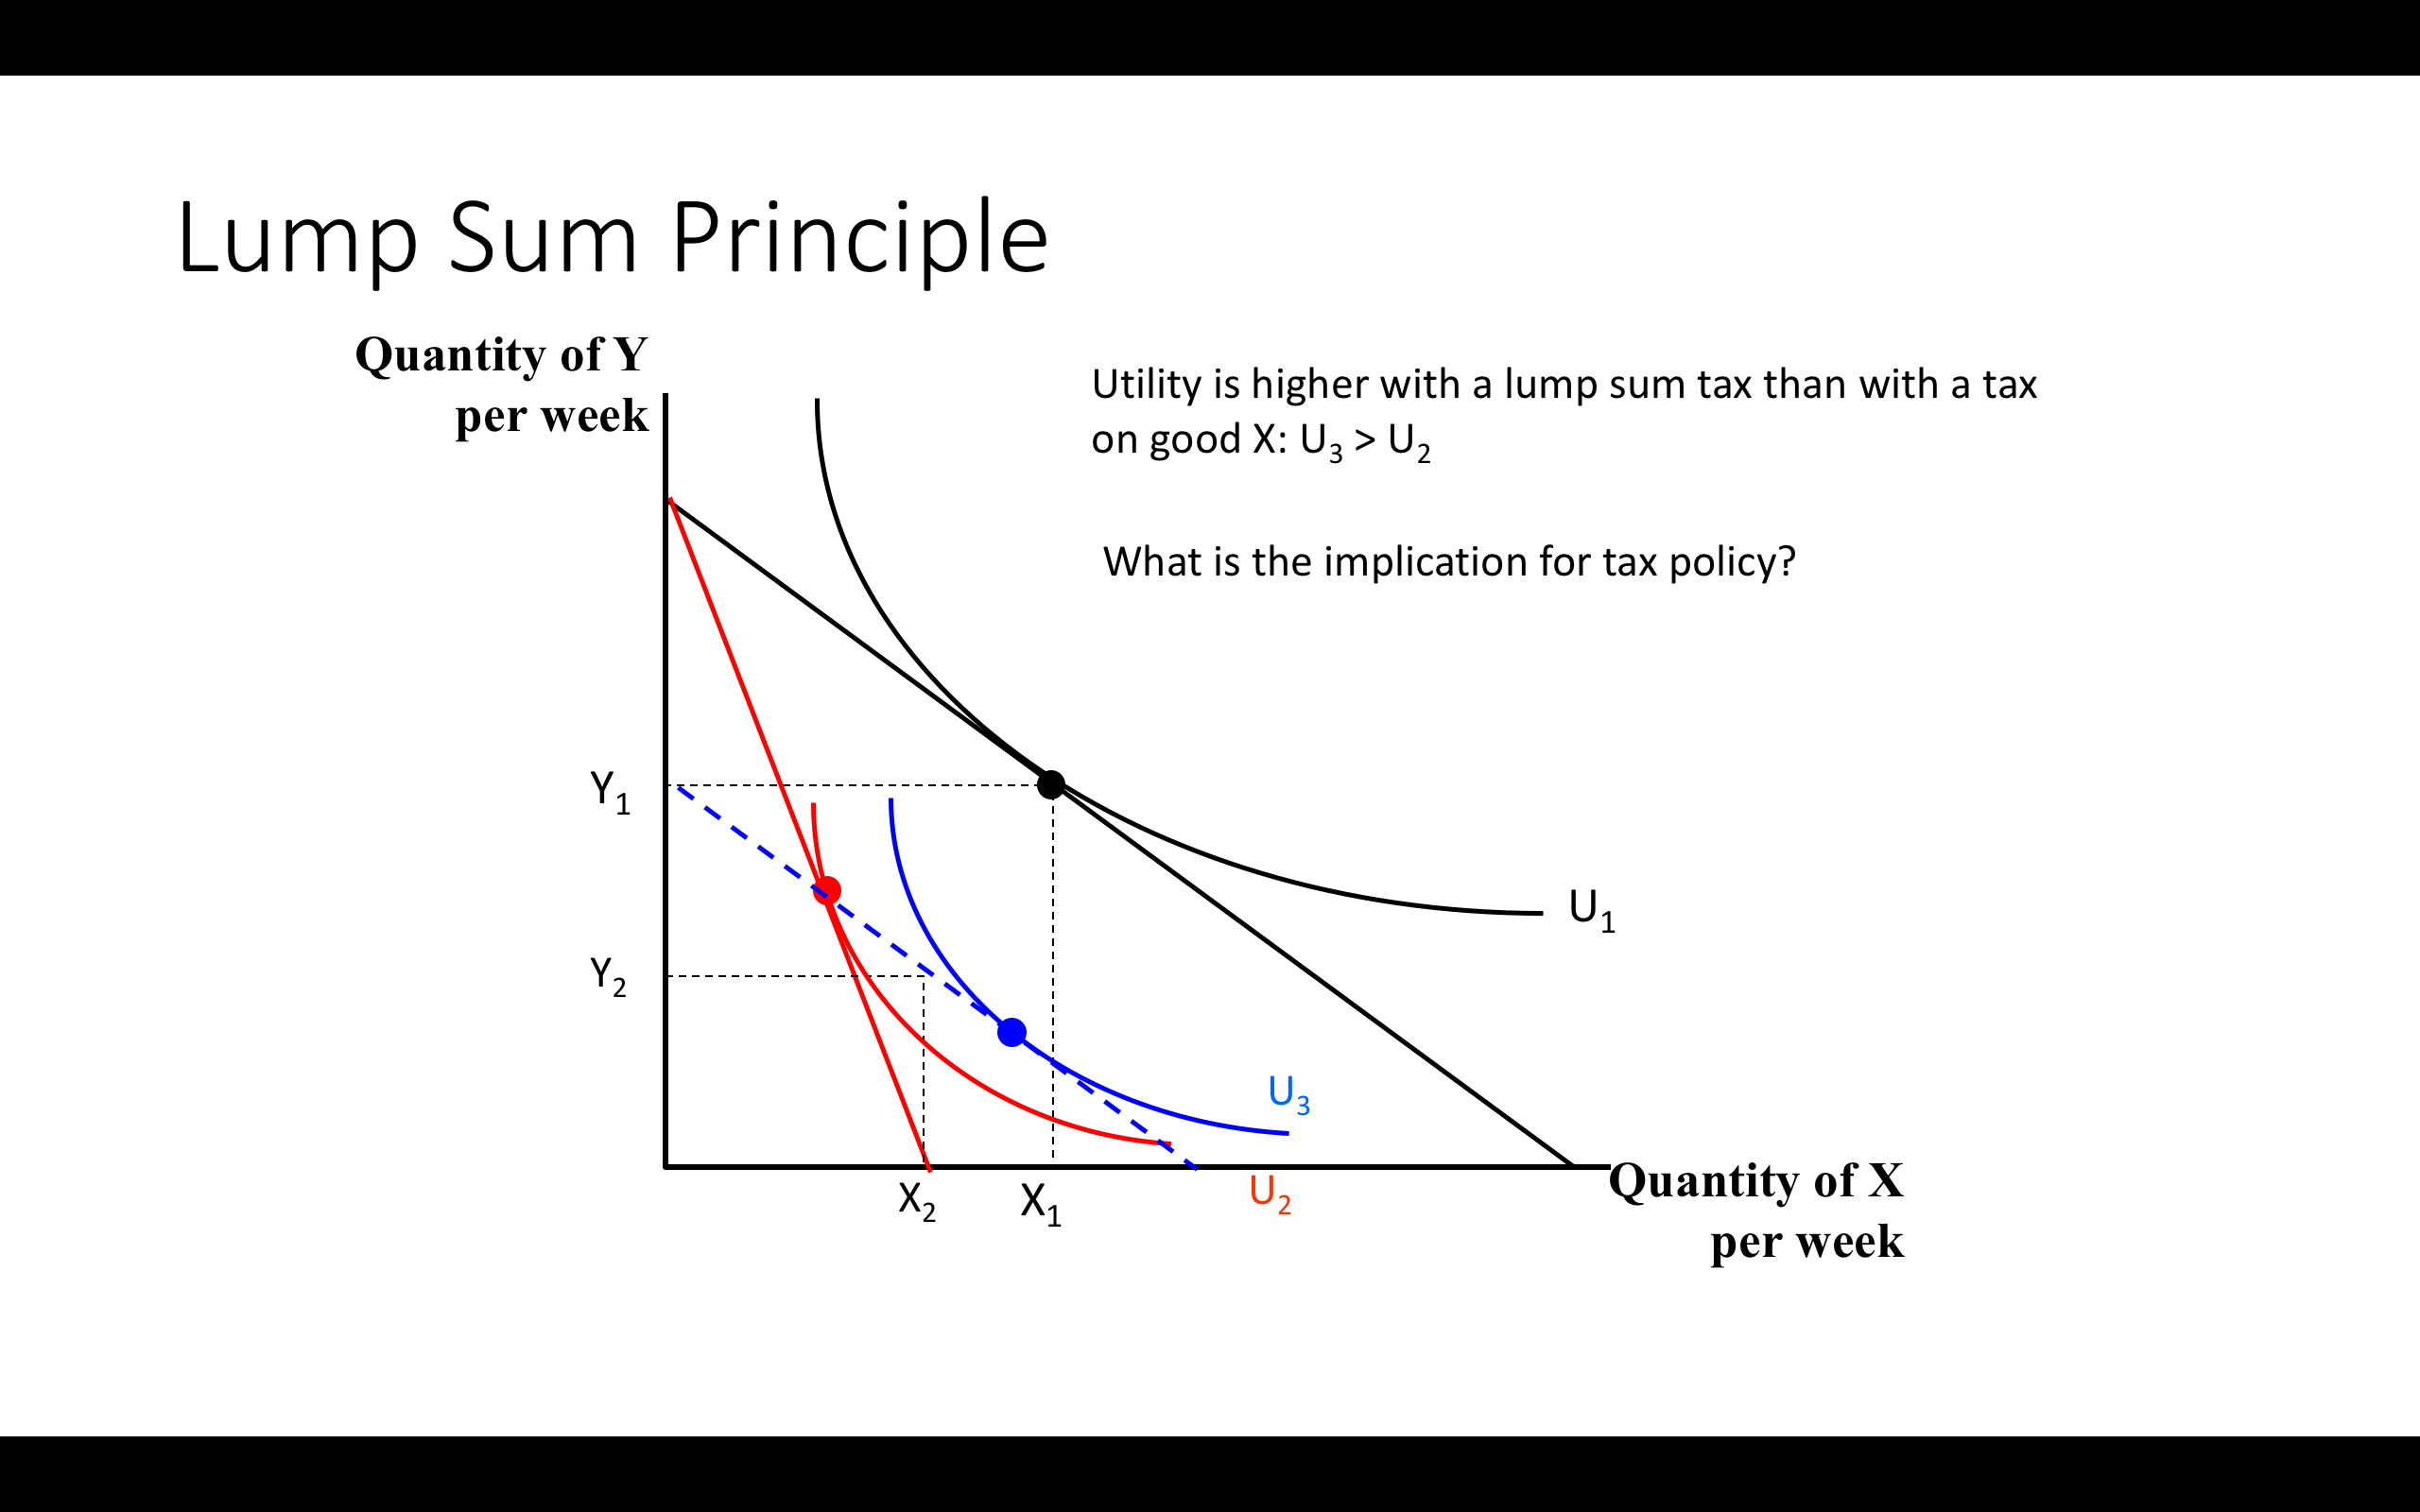
\includegraphics[height=3.3in]{picsfigs/lumpsum2.png}

\pdfnote{Just a single example; to see that this *does* hold generally, take Public Economics.}

\pdfnote{Key to understanding: how do we see that the blue and red dot both *raise the same revenue*?}

\pdfnote{Caveat: If you *can't* tax one good (e.g., leisure) \textCR
 you don't want to tax all other goods equally. \textCR
 In general, tax goods that distort behaviour less overall. }

\begin{center}\rule{0.5\linewidth}{\linethickness}\end{center}

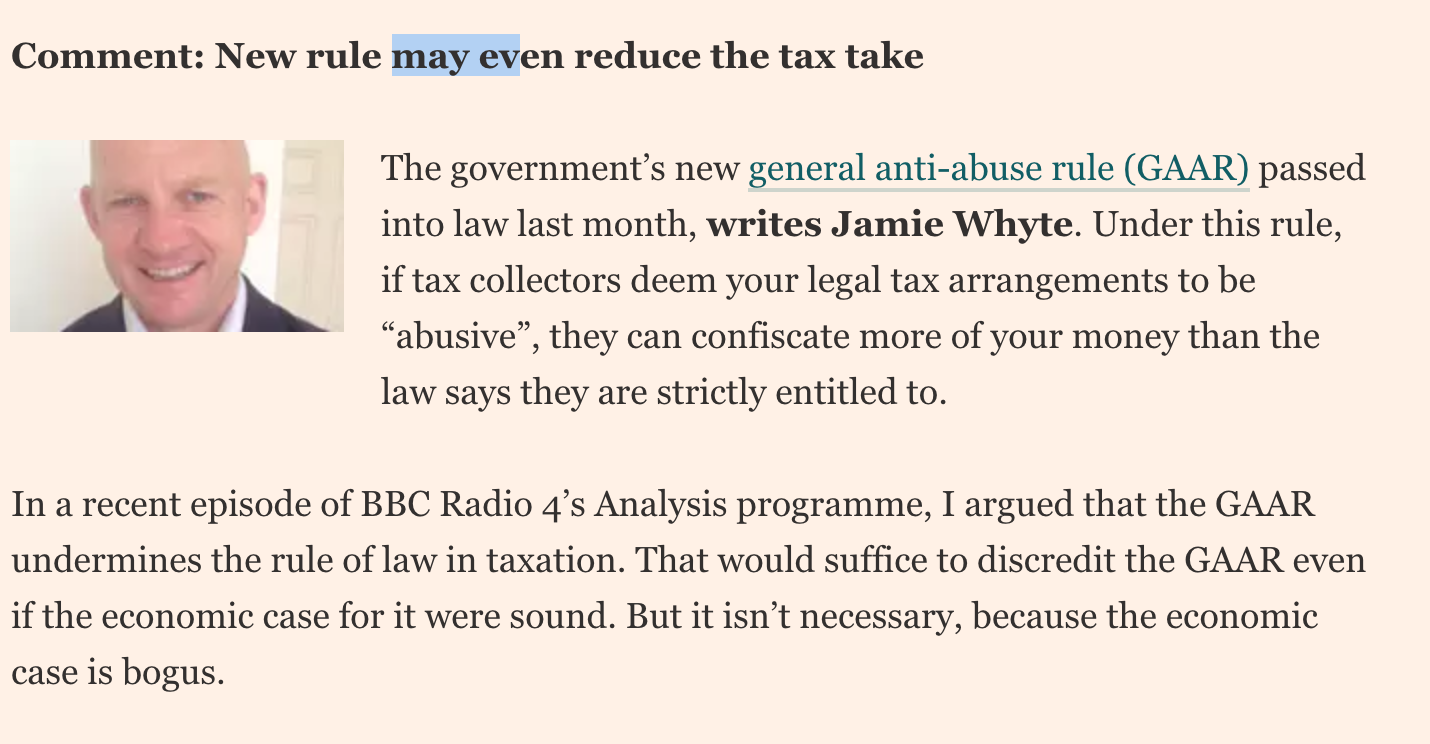
\includegraphics[height=3in]{picsfigs/gaarcomment.png}

\begin{center}\rule{0.5\linewidth}{\linethickness}\end{center}

\href{https://www.ft.com/content/4ea6ab2c-f900-11e2-86e1-00144feabdc0}{FT
Comment: New rule may even reduce the tax take}

\begin{quote}
Suppose I am willing to sell a widget I manufacture for £10 and that you
are willing to spend £11 to own it. Then we will do business and I will
receive a consumer surplus of £1. Now suppose the government imposes a
20 per cent sales tax, and the price I charge for widgets increases to
£12. Since £11 is your maximum price, you won't buy it and the £1 of
consumer surplus you would have gained is lost.
\end{quote}

\begin{quote}
This is how tax avoidance imposes a so-called deadweight cost on
society. People avoid doing valuable things that they would have done if
not for the tax.
\end{quote}

\begin{center}\rule{0.5\linewidth}{\linethickness}\end{center}

\textbf{Read on your own, know:}

\begin{itemize}
\item
  Potential inefficiency of in-kind programmes and subsidies (App 3.3)

  \begin{itemize}
  \tightlist
  \item
    On the other hand, the \emph{benefits} of in-kind programmes rather
    than cash transfers
  \end{itemize}
\end{itemize}

\pdfnote{In  UK,  'welfare wall' called the 'benefits trap' or 'unemployment trap'. \textCR
 This is something succesive governments have tried to remedy; recently with the 'Universal Credit'.}

\pdfnote{Provides an opportunity to *apply* your knowledge to a 'challenge' question}

\hypertarget{changes-in-the-price-of-another-good-what-impact}{%
\subsection{Changes in the Price of Another Good -- what
impact?}\label{changes-in-the-price-of-another-good-what-impact}}

\pdfnote{Previous 2-good diagrams: 'mechanical' impact of the change in $P_X$ on $Y$ \textCR \
- New budget constraint and new $X$ $\rightarrow$ spend the remainder on $Y$. \textCR \
- With 3 or more goods, it's more interesting}

. . .

\begin{description}
\tightlist
\item[Complements]
If rise in \(p_x\) \(\rightarrow\) \(q_{d,y}\) decreases (\& v/v), goods
y and x are \textcolor{gray}{(gross)} \emph{complements} to one another.
\end{description}

\pdfnote{Remember: 'complements' go together --> q-demanded of both responds in same direction to price \textCR
 -- the opposite direction as the price change (unless Giffen).}

\textcolor{gray}{These 'cross-price effects' include both \emph{substitution} and \emph{income} effects. (Hence 'gross'. See micro quiz 3.3).}

. . .

\begin{description}
\tightlist
\item[Substitutes]
If \(p_x\) \(\uparrow\) \(\rightarrow\) \(q_{d,y}\) \(\uparrow\) (and
vice-versa), goods y and x are \textcolor{gray}{(gross)}
\emph{substitutes} \ldots{}
\end{description}

\pdfnote{Rem: 'substitutes' compete to meet same desires, so when you buy more X, buy less Y \textCR
Thus X and Y have *opposite* demand response to a price change in either \textCR
As quantity-demanded for A typically goes *opposite* to P_a \textCR
... q-dmdd for substitute B will go in the *same* direction as the P_a}

\bigskip

\textcolor{red}{Warning:} \(\neq\) `perfect' complements/substitutes

\pdfnote{Here, this is about the *price* reaction, not a fundamental of the utility function.}

\hypertarget{individual-demand-curves}{%
\subsection{Individual demand curves}\label{individual-demand-curves}}

\[d_x(p_x,p_y,I; \: preferences)\]

\begin{itemize}
\tightlist
\item
  `Individual demand curve': plots \emph{individual's} purchase of a
  good versus it's price
\end{itemize}

. . .

\begin{itemize}
\tightlist
\item
  `Map it out': increase \(p_x\) \(\rightarrow\), budget constraint
  shifts inwards \(\rightarrow\)

  \begin{itemize}
  \tightlist
  \item
    New point tangent to indifference curve
  \end{itemize}
\end{itemize}

\begin{center}\rule{0.5\linewidth}{\linethickness}\end{center}

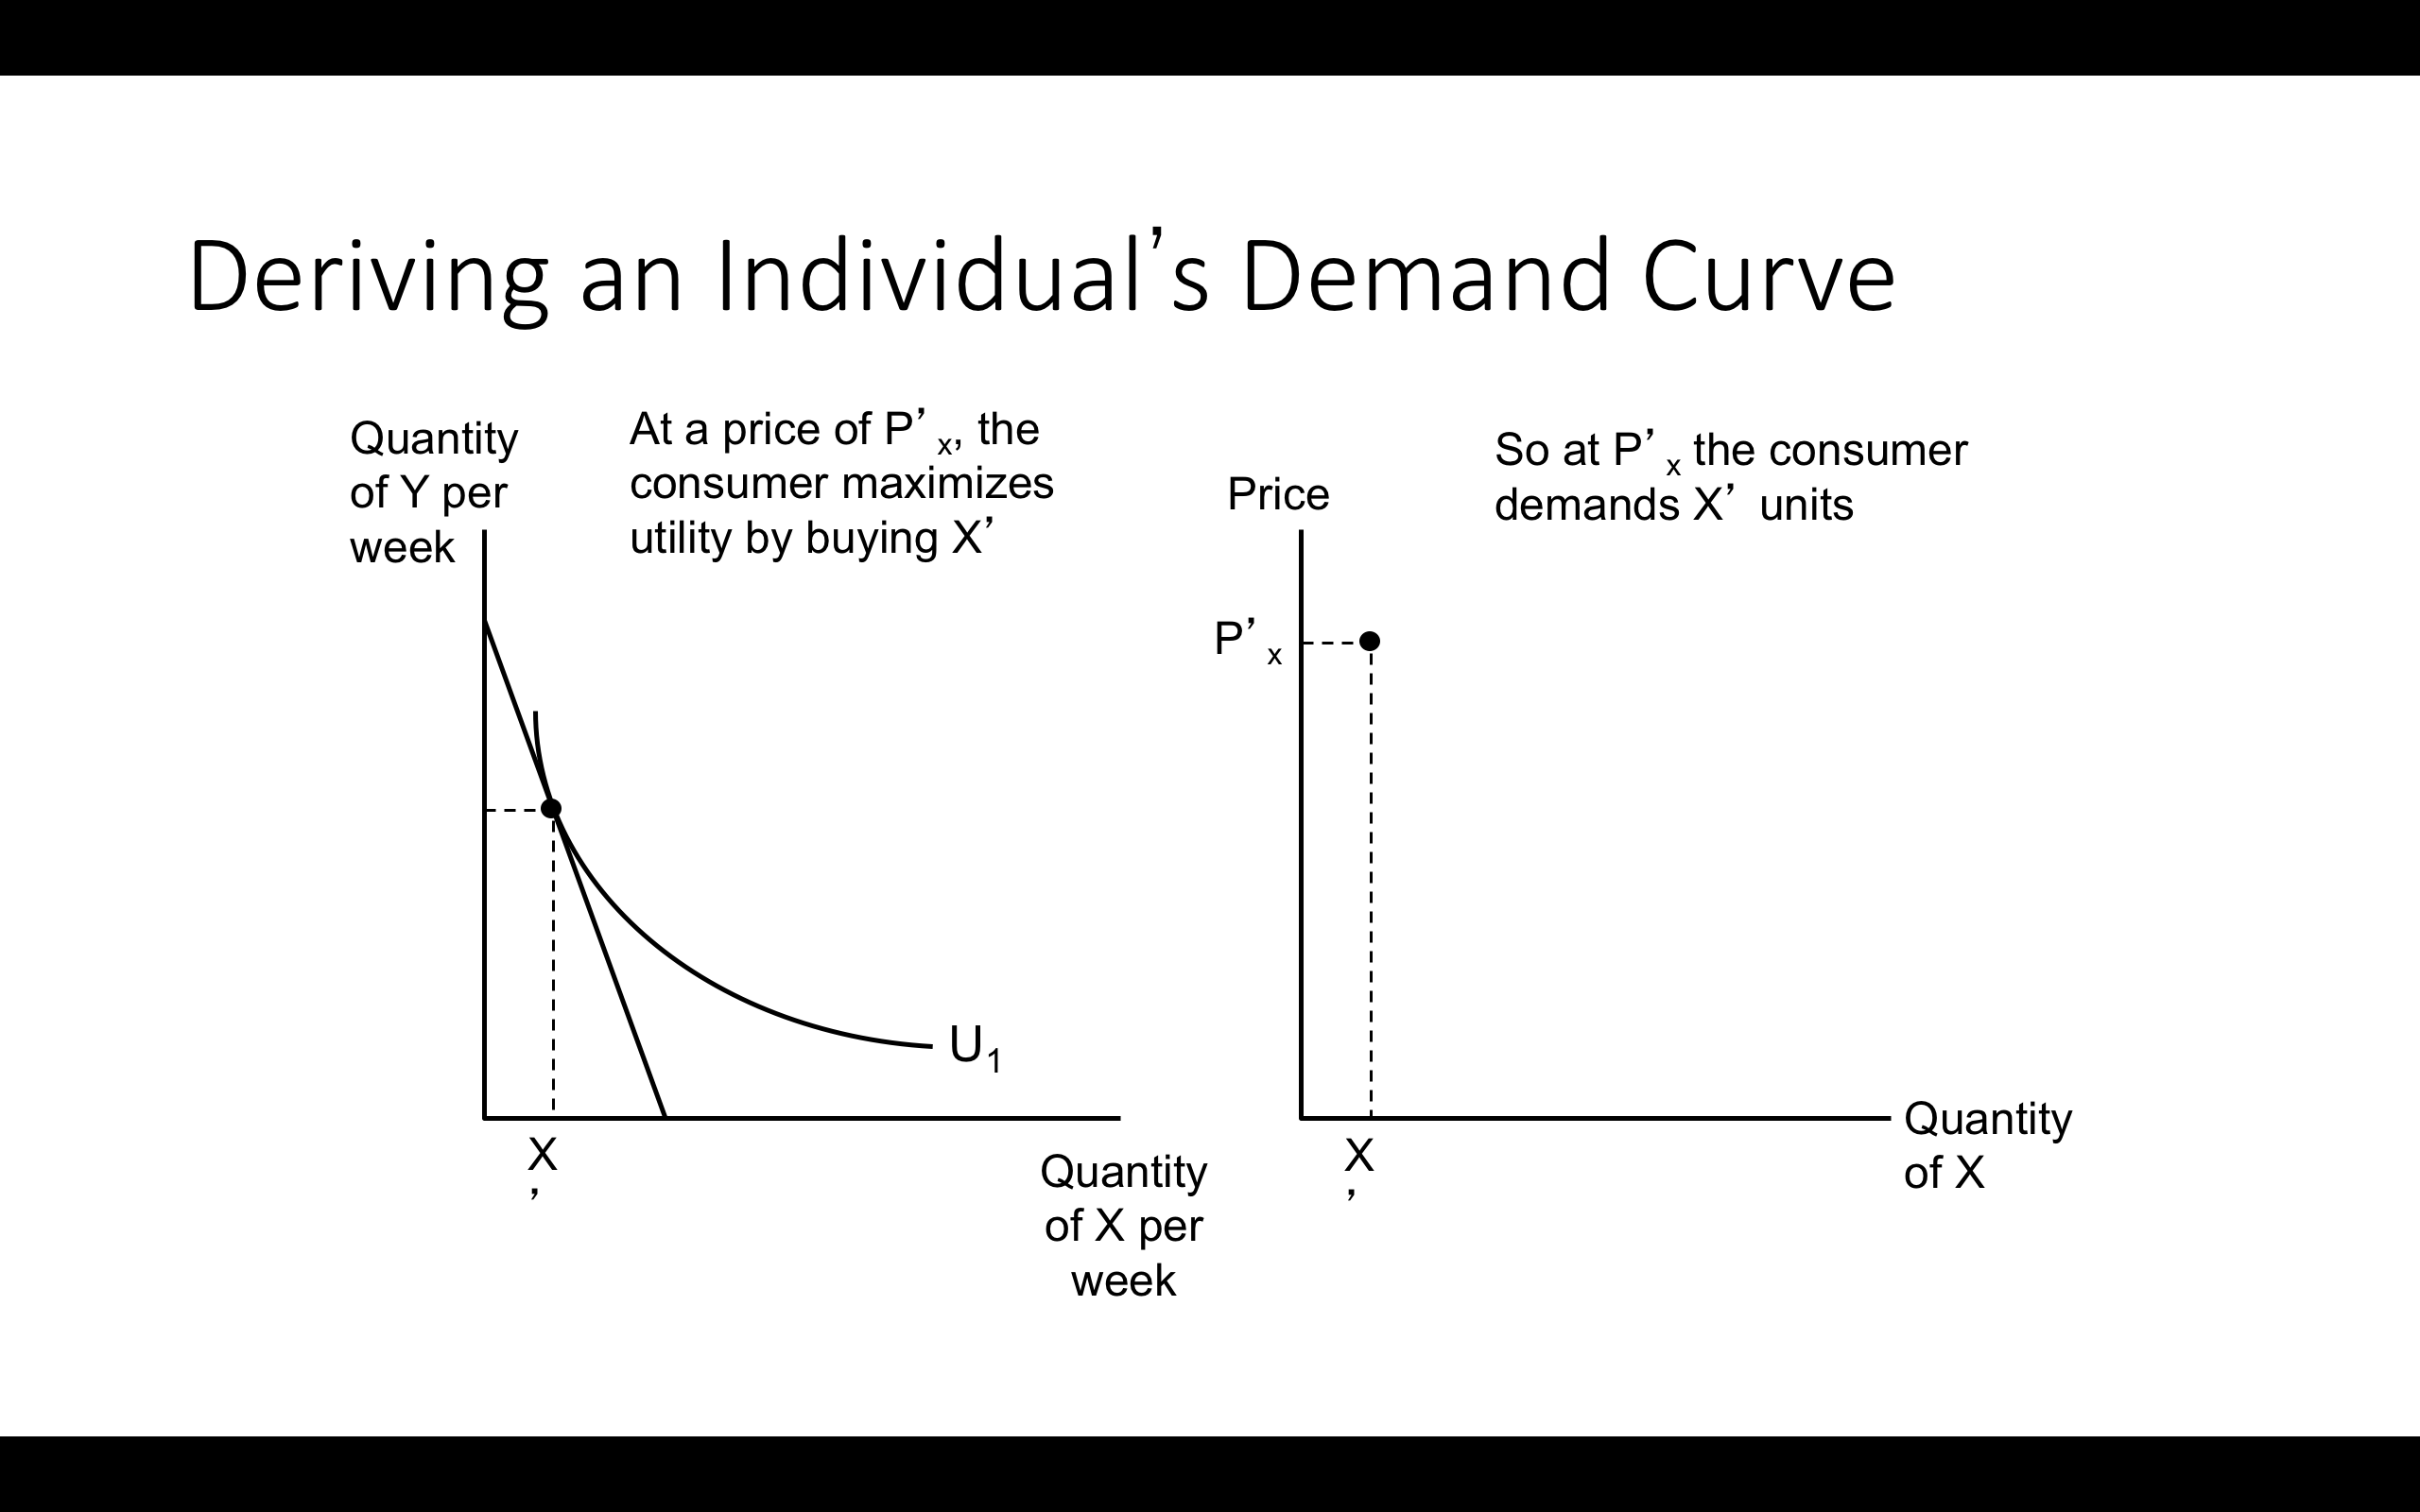
\includegraphics{picsfigs/dmd1.png}\\

\begin{center}\rule{0.5\linewidth}{\linethickness}\end{center}

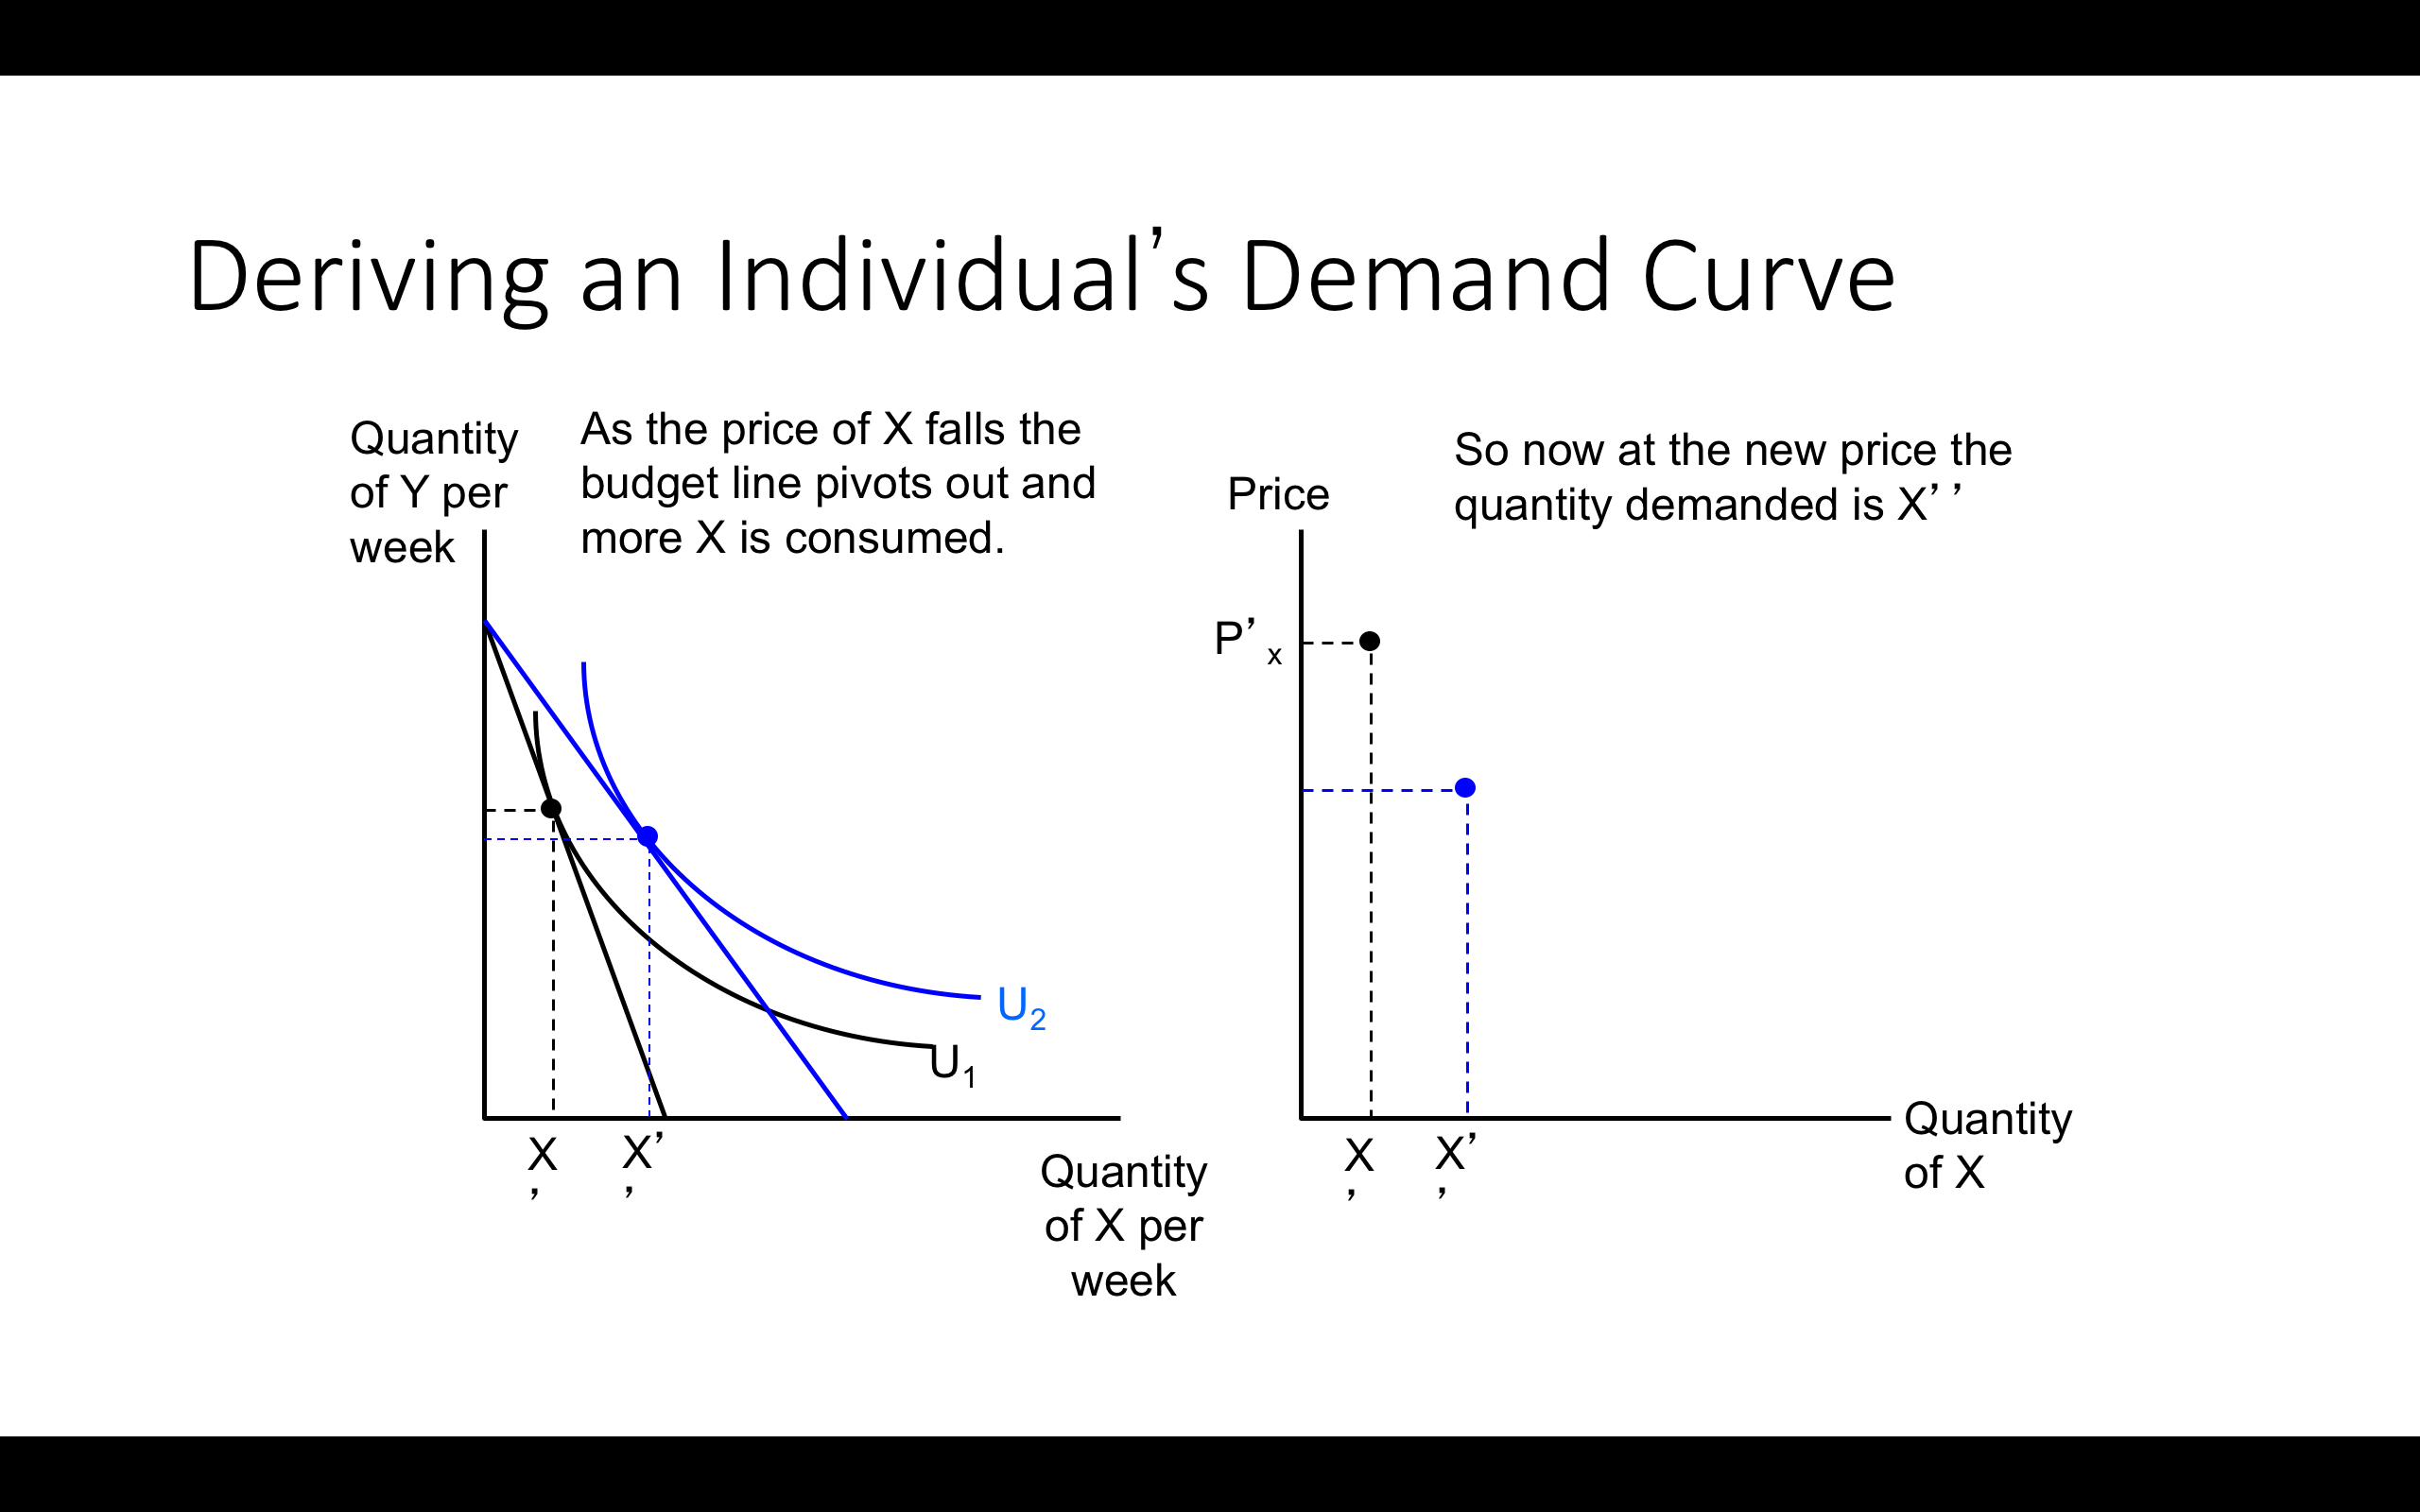
\includegraphics{picsfigs/dmd2.png}\\

\begin{center}\rule{0.5\linewidth}{\linethickness}\end{center}

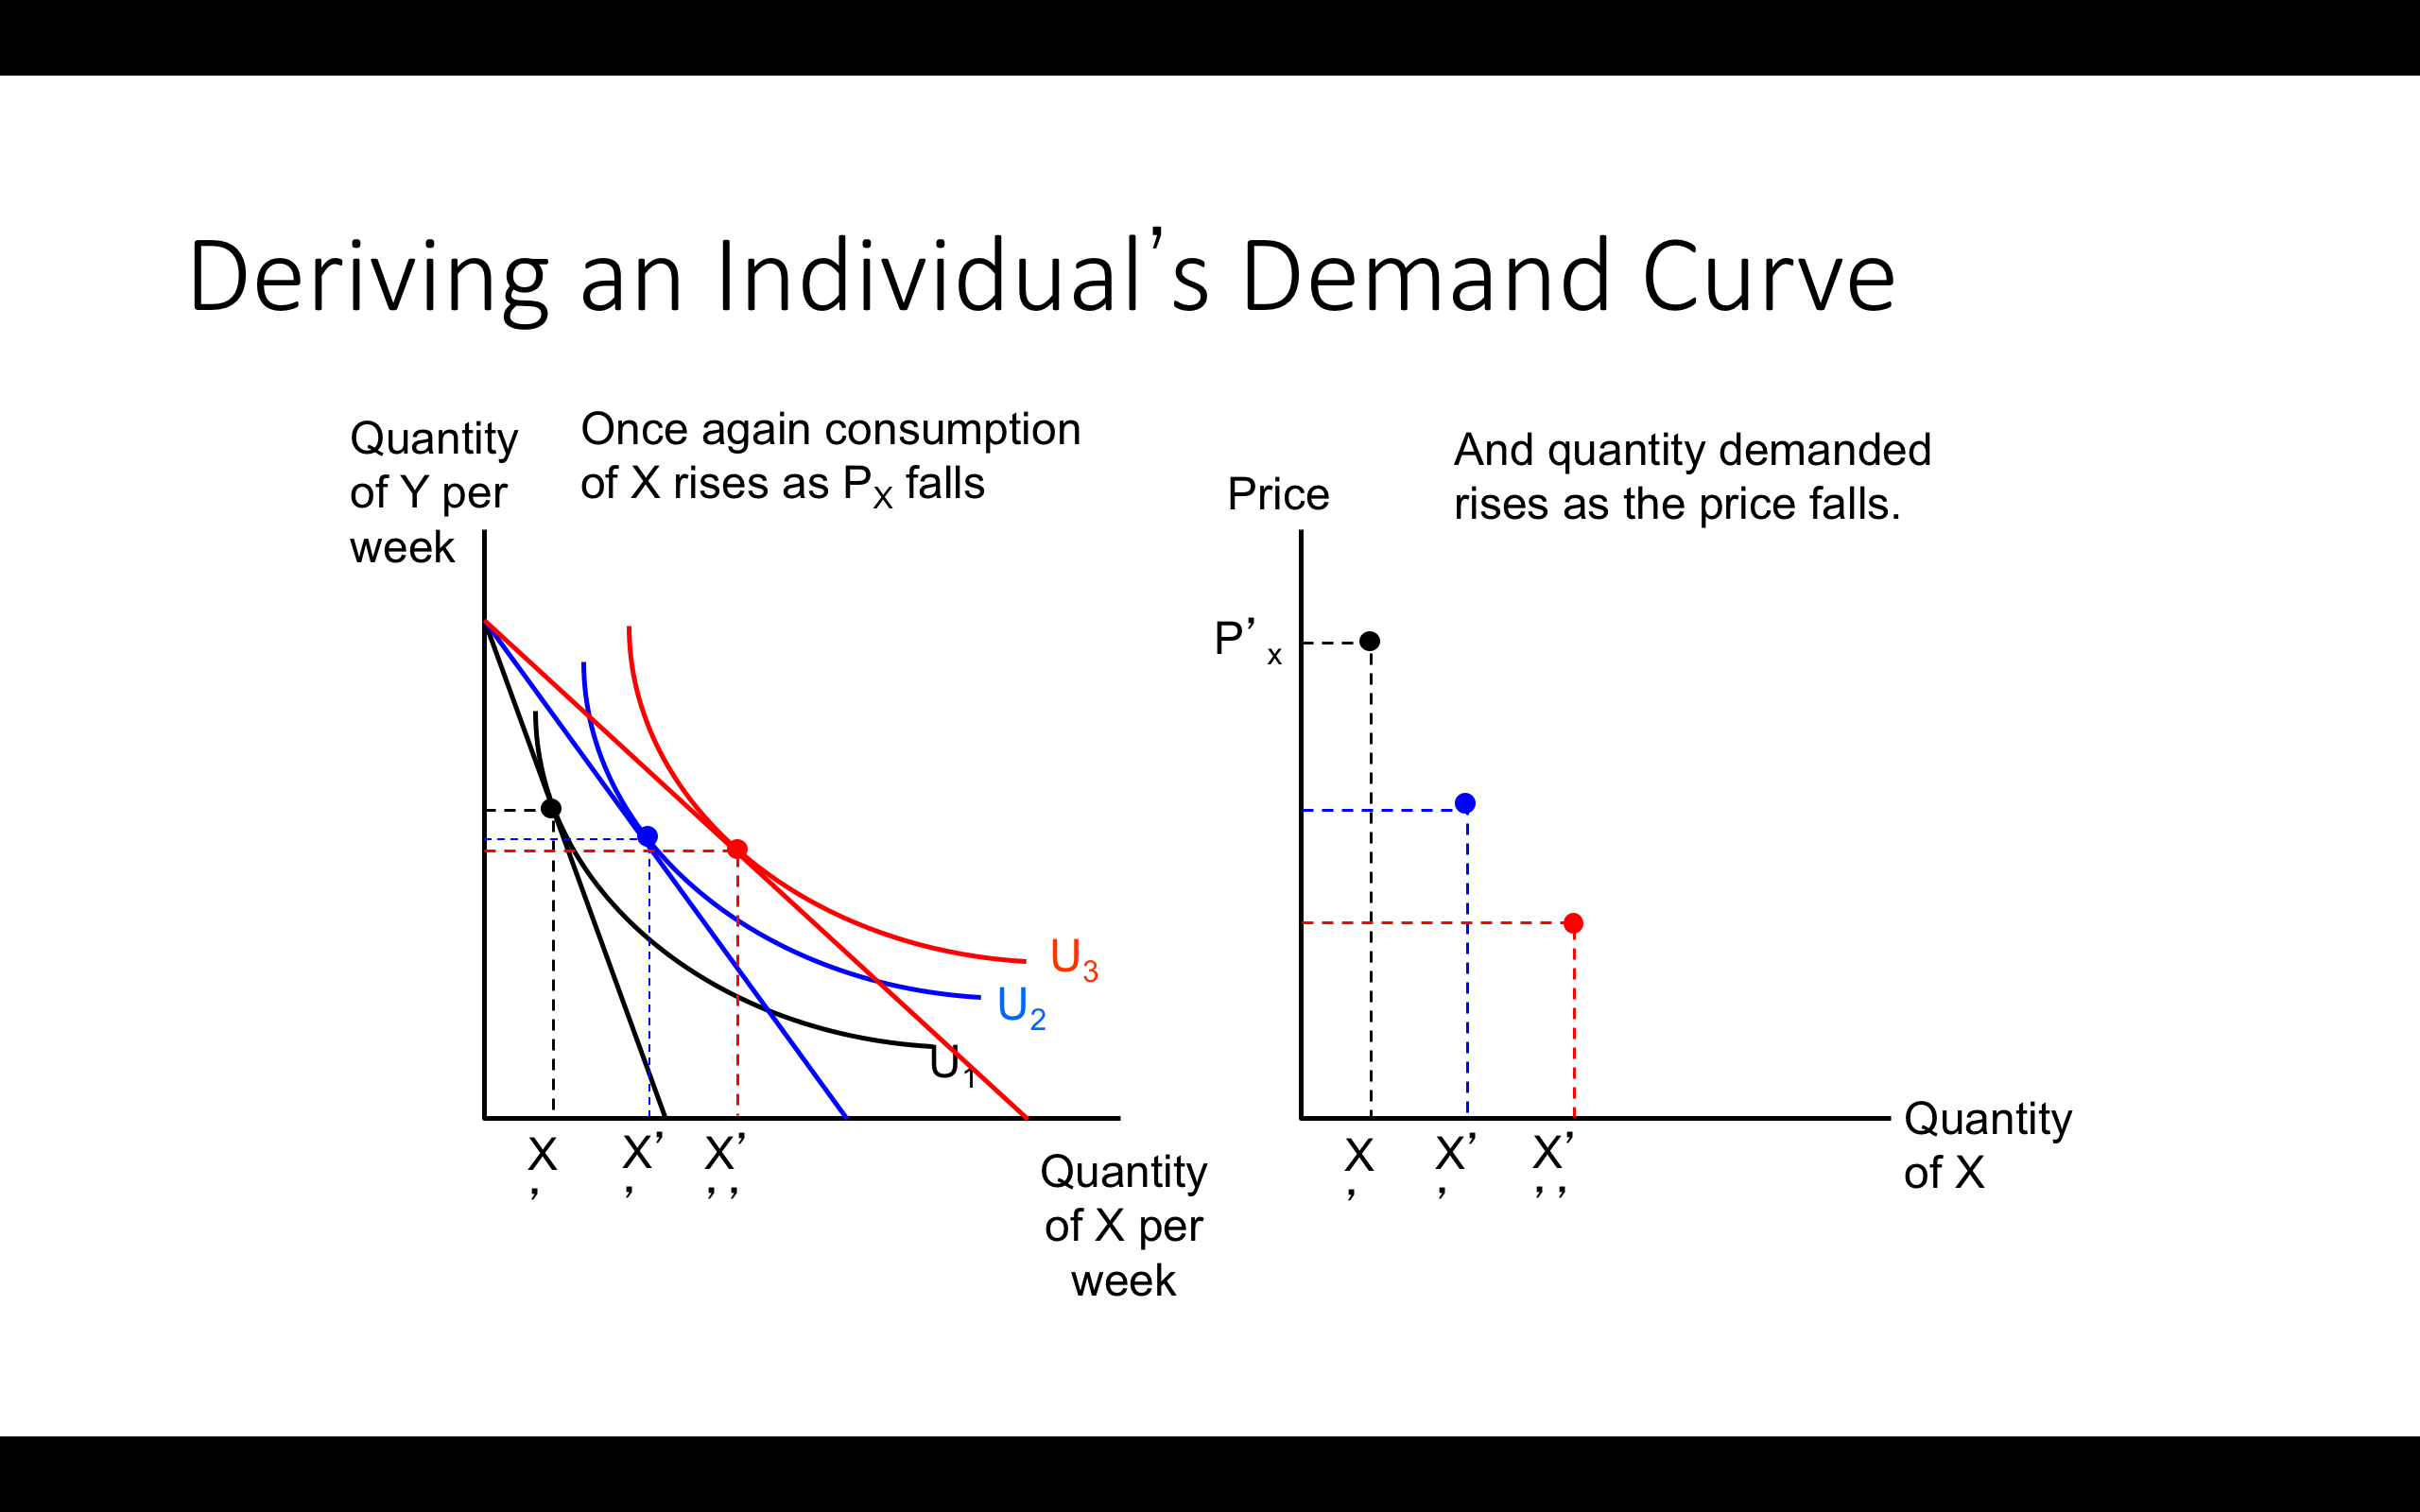
\includegraphics{picsfigs/dmd3.png}\\

\begin{center}\rule{0.5\linewidth}{\linethickness}\end{center}

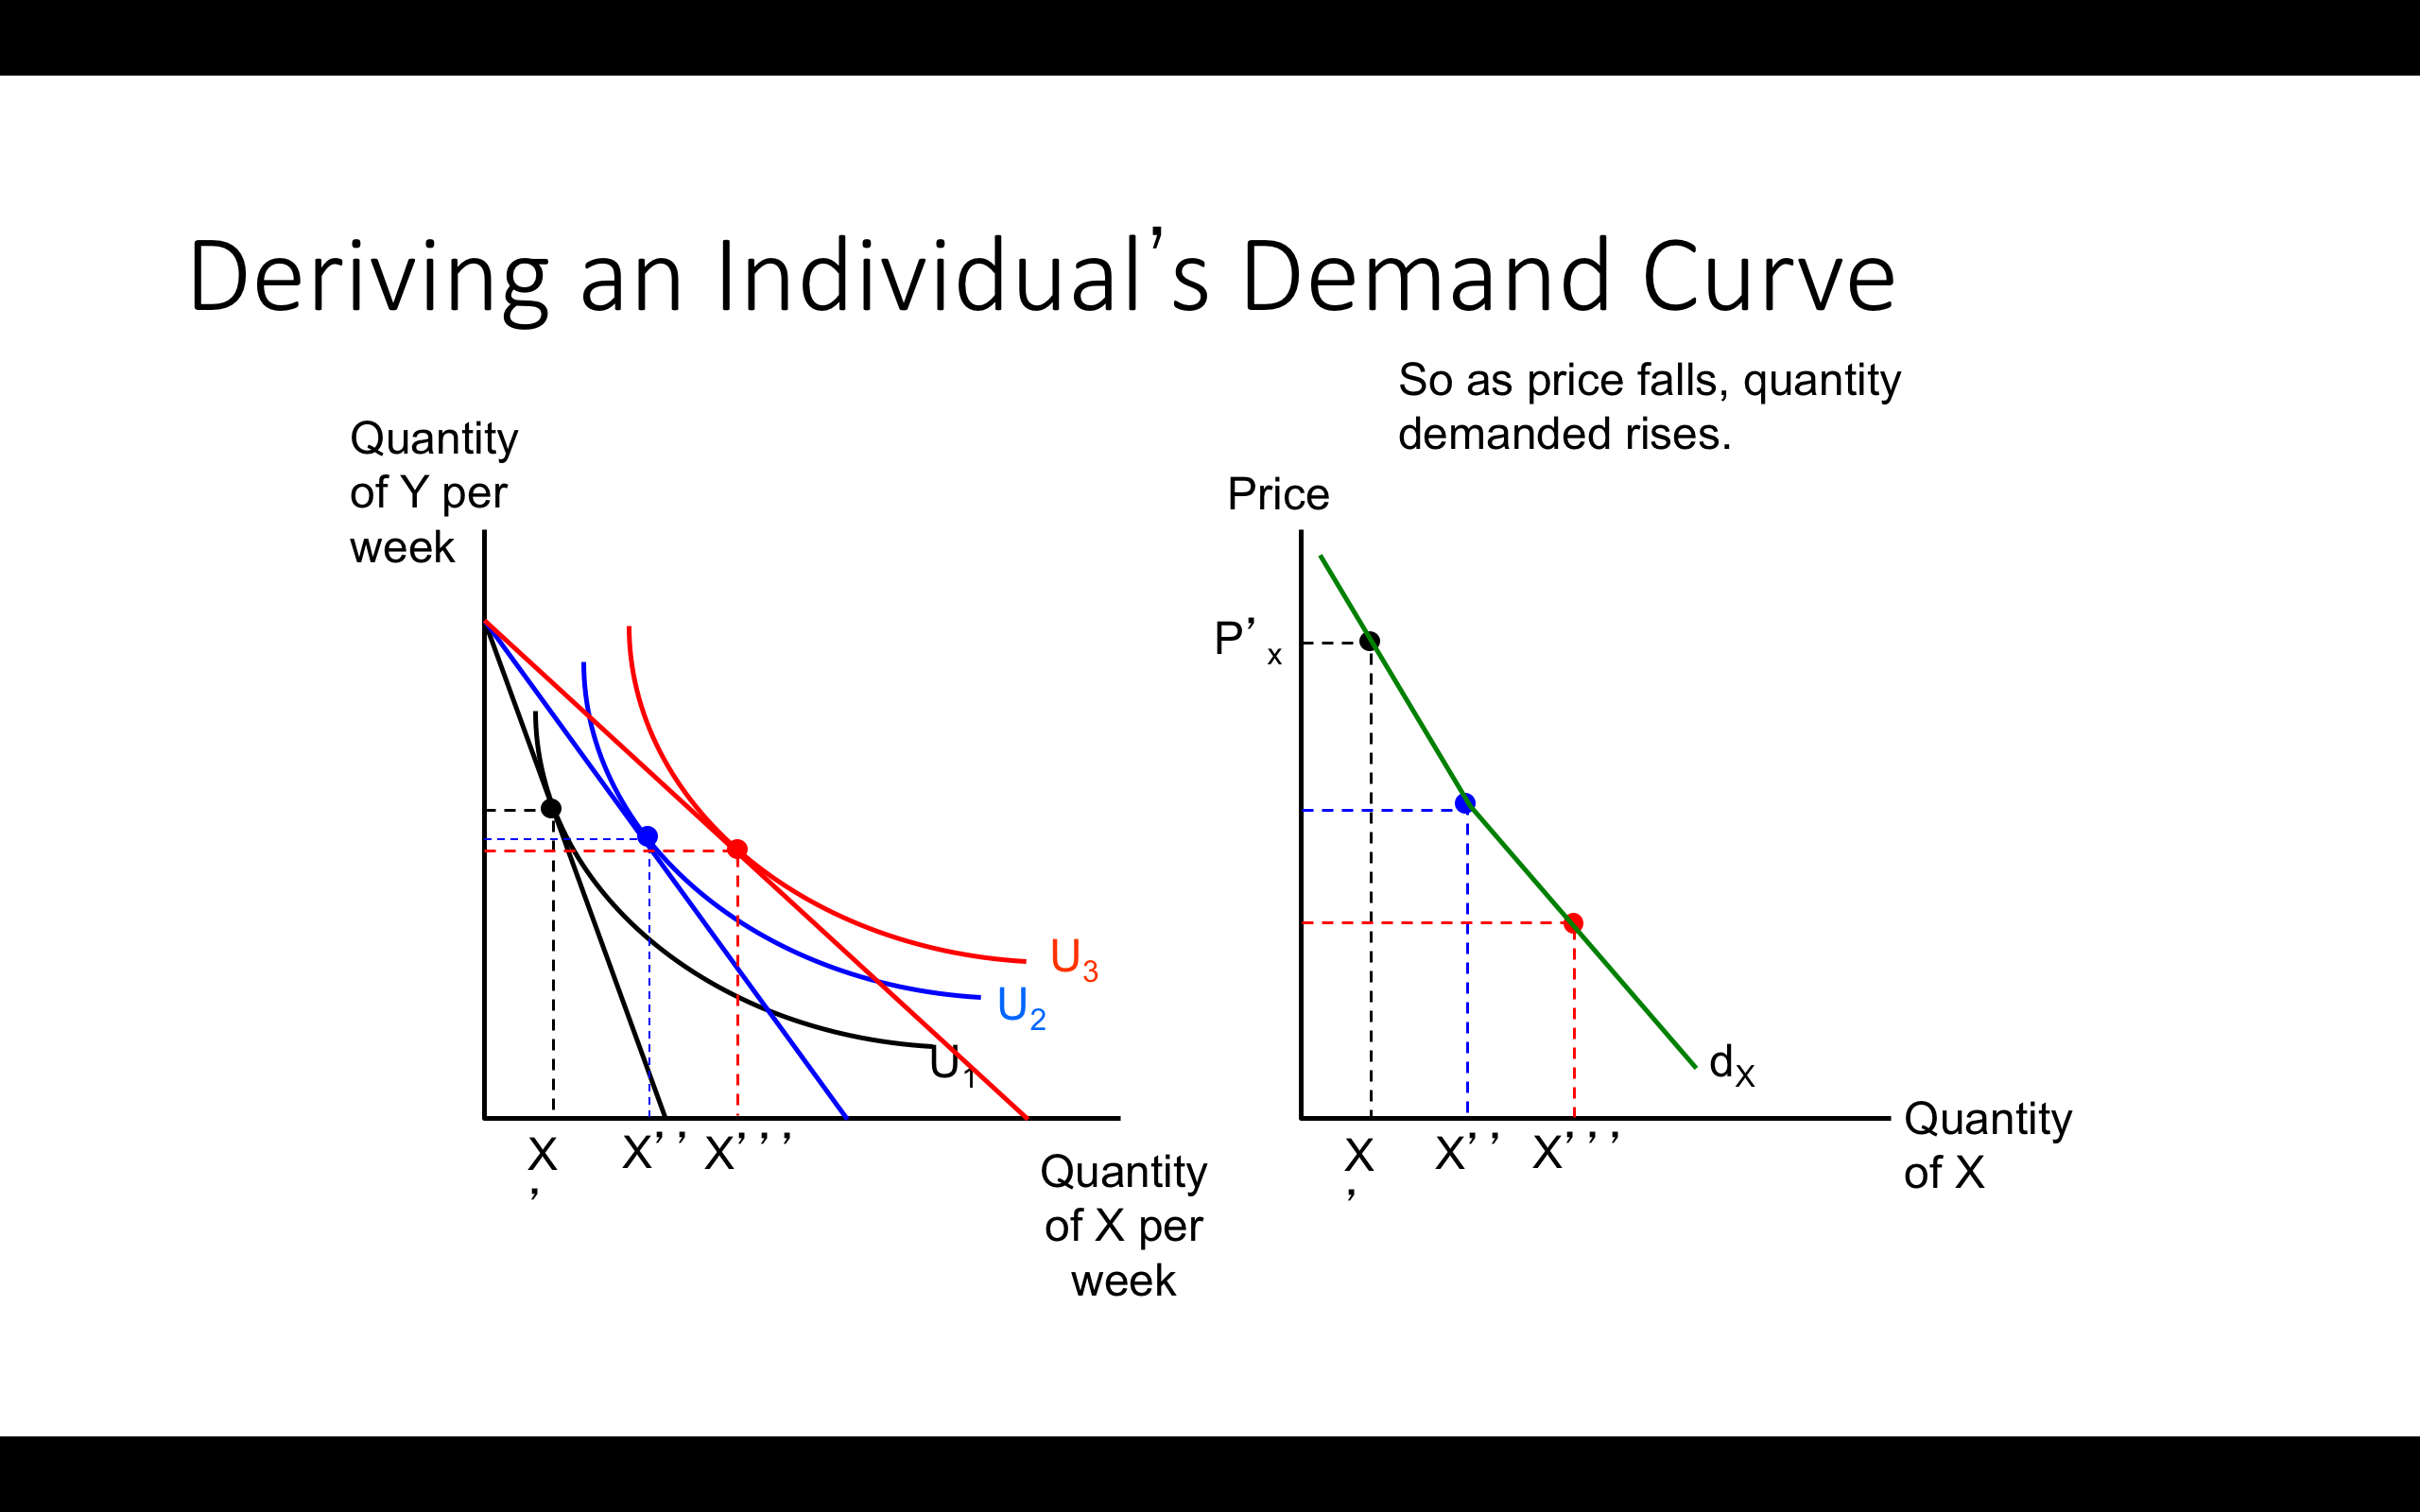
\includegraphics{picsfigs/dmd4.png}\\

\hypertarget{shifts-in-an-individuals-demand-curve}{%
\subsection{Shifts in an individual's demand
curve}\label{shifts-in-an-individuals-demand-curve}}

What might cause an individual's demand curve for a product to shift
(inward or outward)?

. . .

\emph{Not:}

\begin{itemize}
\tightlist
\item
  \emph{Not} `a change in the price of that good'.
\item
  \emph{Not} a shift in the supply curve.
\end{itemize}

. . .

Yes:

\begin{itemize}
\tightlist
\item
  Change in price of complements or substitutes for that good
\item
  Change in income
\item
  Maybe: \(\Delta\) consumer's info, preferences, weather, etc.
\end{itemize}

. . .

\pdfnote{Economists disagree as to how to consider or model changes in preferences}

\textcolor{red}{Be sure you understand shifts vs movements along, and 'a demand curve' vs 'quantity demanded'.}

\pdfnote{Know difference btwn shift in a demand (or supply) curve \& movements along a demand curve, and terminology. \textCR
Almost surely on some exam in some form, see e.g., micro quiz 3.4 \textCR
- Hint: avoid referring to 'supply and demand'; refer to either 'supply and demand *curves*' or 'quantity demanded or supplied'}

\pdfnote{Numerical examples: may be covered in tutorials}

\hypertarget{consumer-surplus}{%
\subsection{Consumer surplus}\label{consumer-surplus}}

\begin{description}
\tightlist
\item[Consumer surplus]
The extra value individuals get from consuming a good over what they pay
for it.
\end{description}

. . .

My wtp for `right to consume good at its current price' (rather than not
at all)

\textcolor{gray}{Measures consumer welfare, used for policy analysis}

. . .

Area between demand curve and market price:

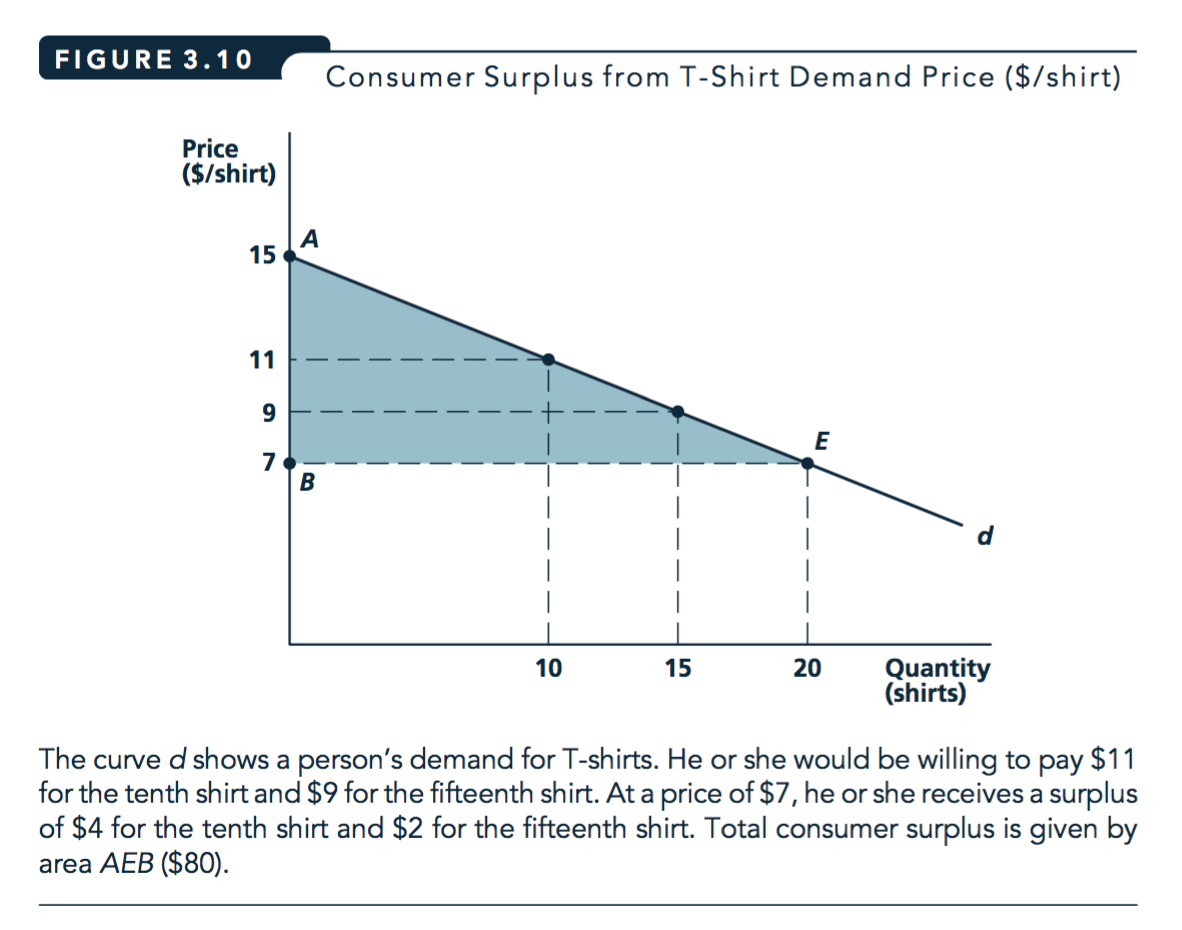
\includegraphics[height=1.6in]{picsfigs/cons_surplus.png}

\pdfnote{Skip section 'consumer surplus and utility' in lecture, but read over it for understanding}

\begin{center}\rule{0.5\linewidth}{\linethickness}\end{center}

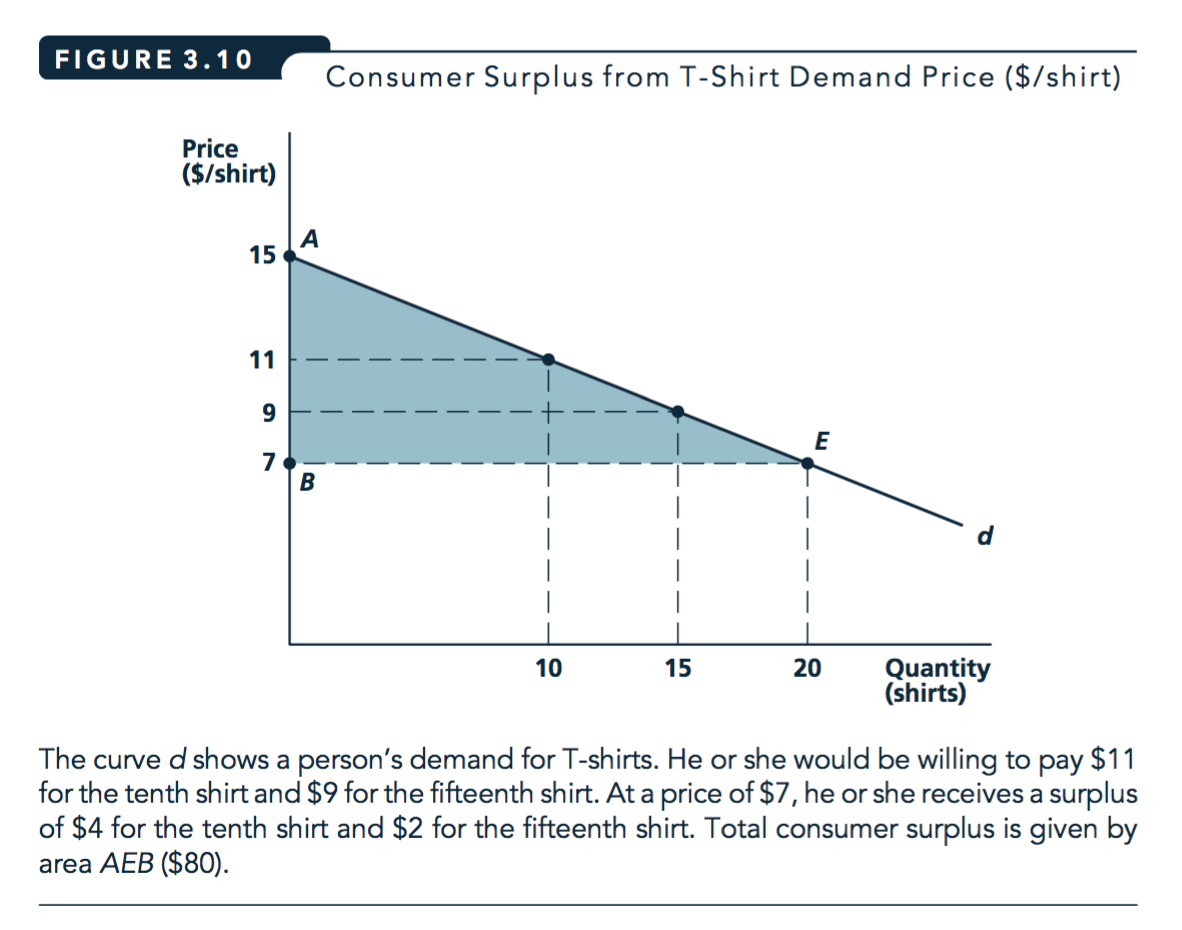
\includegraphics[height=3.5in]{picsfigs/cons_surplus.png}

\pdfnote{Can be applied to the individual or market demand curve to obtain individual or total CS. \textCR
 However, there are some technical issues with the latter.}

\pdfnote{Can also be applied to measuring the value added of a new good (see App 3.4). \textCR
Useful for policy,  e.g.,  subsidies for R\&D, adjusting  CPI; compute damages for 'stifling innovation'}

\begin{description}
\tightlist
\item[Market demand]
Total quantity of a good demanded by all consumers
\end{description}

\begin{itemize}
\tightlist
\item
  Sum individual quantities demanded (at a given price)
\end{itemize}

. . .

\begin{description}
\tightlist
\item[Market demand curve]
Relationship between total quantity demanded of a good and its price,
ceteris paribus
\end{description}

\pdfnote{Some results about individual demand also hold for market demand \textCR
others don't, or only if we make restrictive assumptions}

\begin{center}\rule{0.5\linewidth}{\linethickness}\end{center}

\begin{description}
\tightlist
\item[Market demand curve]
Relationship between total quantity demanded of a good and its price,
ceteris paribus
\end{description}

\begin{itemize}
\tightlist
\item
  Sum the individual demand curves `horizontally' \ldots{} quantities
  demanded at each price
\end{itemize}

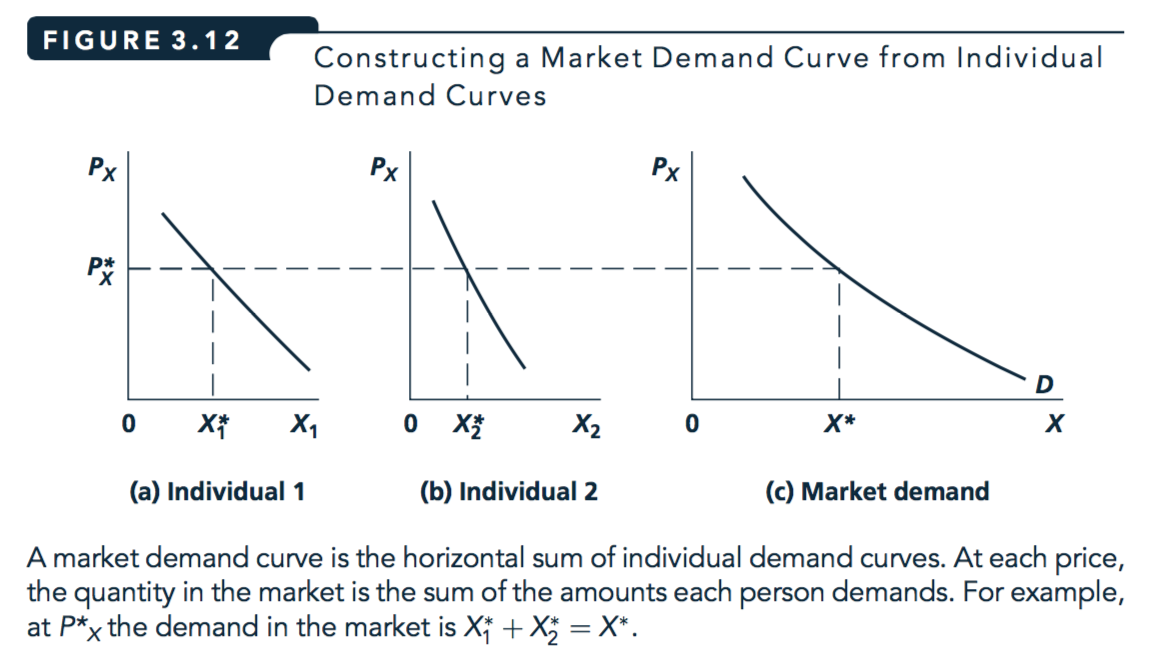
\includegraphics[height=2.3in]{picsfigs/summarketdemandcurve.png}

\pdfnote{Numerical examples of this may be covered in tutorial}
\pdfnote{LC: Illustrate 'sums horizontally' on visualiser if possible}
\pdfnote{Yes, you can add functions.}

\hypertarget{shifts-in-the-market-demand-curve}{%
\subsection{Shifts in the Market Demand
Curve}\label{shifts-in-the-market-demand-curve}}

\begin{itemize}
\tightlist
\item
  Similar things that cause individual demand curve shifts

  \begin{itemize}
  \tightlist
  \item
    Increases in overall income (for normal goods)
  \item
    Reduced prices of complements, increased price of substitutes
  \end{itemize}

  \bigskip
\end{itemize}

\pdfnote{You can only express the demand curve as a function of aggregate income under restrictive assumptions. \textCR
  In general, it depends *who* gets this income. (See 'aggregation issues').}

\begin{center}\rule{0.5\linewidth}{\linethickness}\end{center}

A random example:

\begin{itemize}
\item
  2008: `Gas prices forcing demand for SUVs to plummet'
  \href{http://www.thehour.com/wilton/article/Gas-prices-forcing-demand-for-SUVs-to-plummet-8257785.php}{LINK}
\item
  2015: `Economy, gas prices drive demand for SUVs, high-end cars'
  \href{http://www.sj-r.com/article/20150809/NEWS/150809569}{LINK}
\end{itemize}

\begin{center}\rule{0.5\linewidth}{\linethickness}\end{center}

\hypertarget{elasticities-comparisons-across-contexts}{%
\subsection{Elasticities: comparisons across
contexts}\label{elasticities-comparisons-across-contexts}}

\begin{figure}
   
\includegraphics[height=1.2in]{picsfigs/naveloranges.jpeg}
   
\includegraphics[height=1.2in]{picsfigs/applejuice.jpeg}
\end{figure}

Which is `larger'?:

\begin{itemize}
\item
  change in \(q_d\) of oranges when \(p_{orange}\) rises \emph{or}
\item
  the change in \(q_d\) of apple juice when its price rises?
\end{itemize}

\pdfnote{LC: This is like comparing apples and oranges!}
\pdfnote{Or the response to changes in the price of a related good, or to income.}

. . .

\emph{Difficulty:} Measured in different \emph{units}, p and q have
different starting values!

\begin{center}\rule{0.5\linewidth}{\linethickness}\end{center}

\begin{description}
\item[Elasticity]
the measure of the \% change in one variable brought about by a 1\%
change in another variable.
\end{description}

\begin{itemize}
\tightlist
\item
  a \emph{unitless} measure; will be the same no matter how these
  variables are measured.
\end{itemize}

\pdfnote{Think of responsiveness when talking about elasticity. Actually it's a measure from physics having to do with rubber bands, they tell me.}
\pdfnote{Adv, maths: Strictly speaking we are talking about the limit of these responses, i.e., derivatives. \textCR
  The elasticity is basically the derivative of $ln(y)$ with respect to $ln(x)$; useful to know if you want to run a regression computing an elasticity, or if you want to interpret such a regression.}

\begin{center}\rule{0.5\linewidth}{\linethickness}\end{center}

\begin{itemize}
\item
  If a 5\% fall in the price of oranges typically results in a 10\%
  increase in quantity bought
\item
  we might say that `each percent fall in the price of oranges leads to
  an increase in sales of about 2 percent'
\end{itemize}

. . .

\begin{itemize}
\item
  i.e., the `elasticity' of orange sales wrt price is about 2 \pause

  \begin{itemize}
  \item
    But elasticities need not be constant; they may depend on starting
    point
  \item
    E.g., linear demand \(\rightarrow\) different price elasticity at
    each point
  \end{itemize}
\end{itemize}

\begin{center}\rule{0.5\linewidth}{\linethickness}\end{center}

\hypertarget{price-elasticity-of-demand}{%
\subsection{Price elasticity of
demand}\label{price-elasticity-of-demand}}

Price elasticity of demand:
\[e_{Q_d,p} = \frac{percent \ change \ in \ Q_d}{percent \ change \ in \ p} \]
\[  = \frac{\Delta Q_d}{Q_d}/\frac{\Delta p}{p}\]

\textcolor{gray}{(actually, the limit of this as these changes converge to zero)}

. . .

\begin{itemize}
\item
  Should always be negative (except for Giffen goods)
\item
  A unitless measure related to the slope of the demand curve
\item
  \emph{Very} important for price-setting firms (more on this later)
\end{itemize}

\begin{center}\rule{0.5\linewidth}{\linethickness}\end{center}

\#\#Examples from the headlines

\href{https://www.ft.com/content/2665c794-76a0-11e6-b60a-de4532d5ea35}{India's
Hike Messenger takes aim at WhatsApp}

\begin{quote}
`Reliance ended up showing that there is elasticity in the market. If
you drop prices, people will come on board,' he said.
\end{quote}

\begin{center}\rule{0.5\linewidth}{\linethickness}\end{center}

\href{https://www.ft.com/content/932927d8-266c-3559-b87a-8d3efb07d5e1}{Next
to add more space despite retail sales `moving backwards'}

\begin{quote}
The retailer does not expect any impact from the drop in sterling since
the Brexit vote to kick in until at least the spring of 2017, as it had
hedged some of its foreign-currency exposures in advance. Still, it
expects expenses to rise by up to 5 per cent next year. `The last time
we had to increase prices (which was in 2010 when cotton prices soared)
we estimated that price elasticity was around 1.1.'
\end{quote}

\begin{center}\rule{0.5\linewidth}{\linethickness}\end{center}

\begin{quote}
If that remains the case today, a retail selling price increase of 5\%
would result in a fall in unit sales of -5.5\% and a fall in like for
like sales value of between -0.5\% to -1.0\%. In the scheme of things,
we think that this drag on sales is manageable and less damaging than
taking a significant hit to margin.'
\end{quote}

\begin{center}\rule{0.5\linewidth}{\linethickness}\end{center}

Properties of price elasticity of demand:

\begin{itemize}
\tightlist
\item
  Goods w/ close substitutes at a close price \(\rightarrow\) highly
  elastic
\item
  \ldots{} with few substitutes \ldots{} inelastic
\item
  Typically: elasticity greater in \emph{long run} than short run.
  \textcolor{blue}{Why?}
\end{itemize}

\pdfnote{Ans: Over time, consumers can adjust to price changes by changing their consumption patterns. \textCR
 E.g., if petrol gets more expensive I can switch to a hybrid or electric car, or a bicycle.}

. . .

\begin{longtable}[]{@{}lll@{}}
\toprule
\(e_{Q,p}\) & \(abs(e_{Q,p})\) & Term\tabularnewline
\midrule
\endhead
\(< -1\) & \(>1\) & Elastic\tabularnewline
\(= -1\) & \(=1\) & Unit Elastic\tabularnewline
\(> -1\) & \(<1\) & Inelastic\tabularnewline
\bottomrule
\end{longtable}

\pdfnote{Sometimes elasticities are expressed in absolute value terms (a positive number). It should be clear from the context.}

\begin{center}\rule{0.5\linewidth}{\linethickness}\end{center}

\begin{itemize}
\tightlist
\item
  Total expenditure (revenue): price \(\times\) quantity
\item
  So percent \emph{change} in total expenditure is:

  \begin{itemize}
  \tightlist
  \item
    pct change price \(\times\) pct \emph{change} quantity
  \end{itemize}
\item
  As \(e_{Q,p}\) tells you the pct change quantity for a small pct
  change in price:
\end{itemize}

. . .

\begin{longtable}[]{@{}llll@{}}
\toprule
\(abs(e_{Q,p})\) & Term & p rise \(\rightarrow\) expdr & p falls
\(\rightarrow\) expdr\tabularnewline
\midrule
\endhead
\(>1\) & Elastic & Falls bc Q falls \emph{more} & Rises\tabularnewline
\(=1\) & Unit Elastic & Constant & Constant\tabularnewline
\(<1\) & Inelastic & Rises bc Q falls \emph{less} & Falls\tabularnewline
\bottomrule
\end{longtable}

\pdfnote{Q: A price-setting firm should basically never want to set its price at a point where demand is inelastic. Why not?}

\pdfnote{Ans: If it were at such a point, it could raise its price and its revenue would increase and costs would decline \textCR
 (because it would be selling fewer products but for greater total revenue.) \textCR
 A caveat is that it might do this for a long term strategic advantage; e.g., to gain customer loyalty and market share, intending to take its profits later.}

\begin{center}\rule{0.5\linewidth}{\linethickness}\end{center}

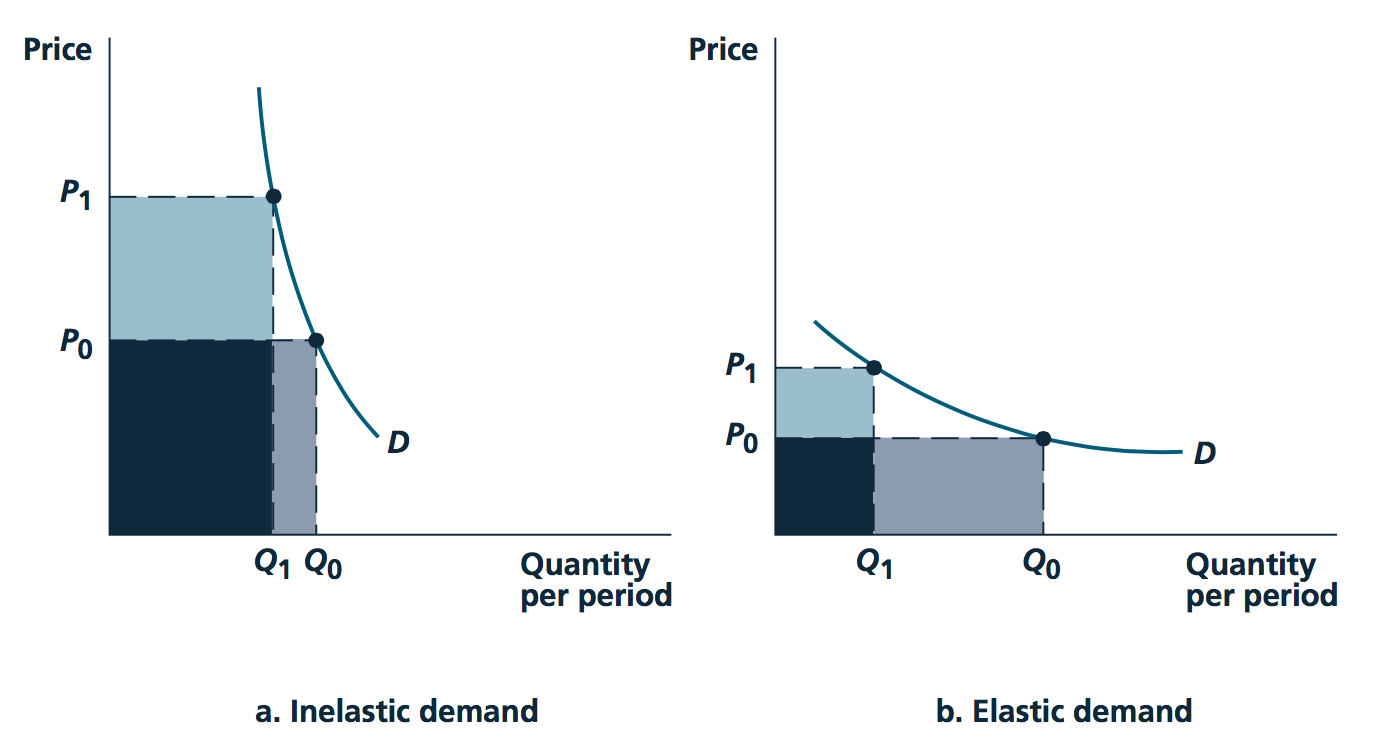
\includegraphics{picsfigs/elast_revenue.png}\\

\hypertarget{next-bits-on-price-elasticity-of-demand}{%
\subsection{Next bits on price elasticity of
demand}\label{next-bits-on-price-elasticity-of-demand}}

\begin{itemize}
\tightlist
\item
  Numerical example (may be covered in tutorial)
\item
  Skip: Unit Elastic Curve
\item
  Read on your own: Application 3.7: An Experiment in Health Insurance
\end{itemize}

\hypertarget{income-elasticity-of-demand}{%
\subsection{Income elasticity of
demand}\label{income-elasticity-of-demand}}

\begin{description}
\tightlist
\item[Income elasticity of demand]
\% change in quantity demanded of a good in response to 1\% change in
income.
\end{description}

\[e_{Q_d,I} = \frac{percent \ change \ in \ Q_d}{percent \ change \ in \  I} \]
\[  = \frac{\Delta Q_d}{Q_d}/\frac{\Delta I}{I}\]\\

. . .

Normal goods: \(e_{Q,I} > 0\)\\

Inferior goods: \(e_{Q,I} < 0\)

. . .

Luxury goods: \(e_{Q,I} > 1\)

\pdfnote{E.g., cocaine is a luxury good, if, when I win /pounds1000 in the lottery, I will increase my consumption of cocaine by *more* than /pounds1000 ... \textCR
 (assuming, as in classical models, that I treat all sources of income the same}

\pdfnote{Q: Is a luxury good a normal good?}
\pdfnote{Ans: Yes, because $1>0$. However, a normal good may or may not be a luxury good.}
\pdfnote{Engel's 'law': As income increases, food becomes a smaller share of income.}

\pdfnote{Q (micro quiz): Why is it that not every good can have an income elasticity of demand greater than 1? \textCR
 Can every good have an income elasticity of demand less than 1?}

\begin{center}\rule{0.5\linewidth}{\linethickness}\end{center}

\href{https://www.ft.com/content/4ea79d96-a4d6-11e5-a91e-162b86790c58}{Prof.~Muellbauer
letter to FT}o

\begin{quote}
Sir, Professor Gordon Gemmill (Letters, December 14), surprisingly for a
trained economist, assumes an income elasticity of demand of zero for
housing: that is, that people do not demand more and better housing as
they become richer. Nowhere in the world is this the case! My own
empirical work demonstrates that around two-thirds of the rise in UK
house prices, corrected for general inflation, since 1980 is because
supply is not keeping up with income and population growth.
\end{quote}

\begin{center}\rule{0.5\linewidth}{\linethickness}\end{center}

\begin{quote}
Other drivers do exist \ldots{} The price effects of extra supply take
time to build up. I agree on that. But just imagine what would happen if
we did nothing more than we are now doing: population and income growth
would drive prices even higher even though we already hold the record
for rises in house prices since 1970 among the group of seven leading
high-income countries. We need to build far more housing, in the right
locations. And we need to start now. - Prof John Muellbauer Nuffield
College, Oxford, UK
\end{quote}

\begin{center}\rule{0.5\linewidth}{\linethickness}\end{center}

\hypertarget{rest-of-chapter-3}{%
\subsection{Rest of chapter 3}\label{rest-of-chapter-3}}

Read on your own:

\begin{itemize}
\item
  Cross-price elasticity of demand (read on your own)
\item
  Some elasticity estimates (note these are a bit dated)
\end{itemize}

\begin{center}\rule{0.5\linewidth}{\linethickness}\end{center}

\hypertarget{tutorial-and-suggested-problems-from-chapter-3-see-vle}{%
\subsection{Tutorial and suggested problems from chapter 3: see
VLE}\label{tutorial-and-suggested-problems-from-chapter-3-see-vle}}


\end{document}
